\documentclass[11pt]{report}
\usepackage[english, german]{babel}
\usepackage{geometry}                % See geometry.pdf to learn the layout options. There are lots.
\geometry{a4paper}                   % ... or a4paper or a5paper or ... 
%\usepackage[parfill]{parskip}    % Activate to begin paragraphs with an empty line rather than an indent
\usepackage{xifthen}
\usepackage{xstring}			% to check content of strings in xifthen
\usepackage{graphicx}
\usepackage{parskip}
\usepackage[usenames,dvipsnames,table]{xcolor}
\usepackage{amssymb}
\usepackage{epstopdf}
\usepackage[utf8]{inputenc}
\usepackage{hyperref}
\usepackage{fancyhdr}
\usepackage{float}
%\usepackage{natbib}
\usepackage{url}

\newcommand{\titleofthesis}{Mesh Netzwerk}
\newcommand{\department}{Informatik} % Replace by your department

\newcommand{\firstauthor}{Tim Untersberger}
\newcommand{\firstauthorclass}{5BHIF}
\newcommand{\secondauthor}{Stefan Waldl}
\newcommand{\secondauthorclass}{5BHIF}

\newcommand{\duedateen}{April 3, 2020} % due date in english format
\newcommand{\duedatede}{3. April 2020} % due date in german format
\newcommand{\supervisor}{Thomas Stütz, Gerald Köck}
\newcommand{\projectpartner}{HTBLA Leonding}
 % Set basic data (author, title, etc.) of your thesis
\IfStrEq*{\languagename}{english}
	{
		\newcommand{\dalabel}{Diploma Thesis}
		\newcommand{\submittedlabel}{Submitted by}
		\newcommand{\datelabel}{Date}
		\newcommand{\duedatevalue}{\duedateen}
		\newcommand{\supervisorlabel}{Supervisor}
		\newcommand{\projectpartnerlabel}{Project Partner}
	}
	{
		\newcommand{\dalabel}{Diplomarbeit}
		\newcommand{\submittedlabel}{Eingereicht von}
		\newcommand{\datelabel}{Datum}
		\newcommand{\duedatevalue}{\duedatede}
		\newcommand{\supervisorlabel}{Betreuer}
		\newcommand{\projectpartnerlabel}{Projektpartner}
	}
 % This file should not really be touched

\begin{document}
\rhead{
\includegraphics[scale=.9]{images/Logo.png}}
\cfoot{}
\begin{titlepage}
\thispagestyle{fancy}

\begin{center}

\vspace*{8em}

{\LARGE \dalabel}

\vspace{2em}

{\large Höhere Technische Bundeslehranstalt Leonding \\[.5em]
Abteilung für \department}

%\vspace{8em}
\vspace*{\fill}

{\Huge \titleofthesis}
\end{center}

%\vspace{8em}
\vspace*{\fill}

\begin{tabular}{ll}
\ifthenelse{\isundefined{\firstauthor}}{}{\submittedlabel: & {\bf \firstauthor, \firstauthorclass}}
\ifthenelse{\isundefined{\secondauthor}}{}{ \\[.5em] & {\bf \secondauthor, \secondauthorclass}}
\ifthenelse{\isundefined{\thirdauthor}}{}{ \\[.5em] & {\bf \thirdauthor, \thirdauthorclass}}
\ifthenelse{\isundefined{\fourthauthor}}{}{ \\[.5em] & {\bf \fourthauthor, \fourthauthorclass}}
 \\[.5em]
\datelabel: & {\bf \duedatevalue} \\[.5em]

\supervisorlabel: & {\bf \supervisor} \\[.5em]

\ifthenelse{\isundefined{\projectpartner}}{}{\projectpartnerlabel: & {\bf \projectpartner}}
\end{tabular}
\end{titlepage}
 % Should not be necessary to touch this file
\section*{Gendererklärung}

Zur besseren Lesbarkeit werden auf dieser Website personenbezogene Bezeichnungen, die sich zugleich auf Frauen und Männer beziehen, generell nur in der im Deutschen üblichen männlichen Form angeführt, also z.B. \glqq Teilnehmer\grqq{} statt \glqq TeilnehmerInnen\grqq{} oder \glqq Teilnehmerinnen und Teilnehmer\grqq{}.

Dies soll jedoch keinesfalls eine Geschlechterdiskriminierung oder eine Verletzung des Gleichheitsgrundsatzes zum Ausdruck bringen.

\section*{Gender Declaration}

For better readability, personal names that refer to women and men at the same time are generally only given in the masculine form common in German, e.g. \glqq Participants\grqq{} instead of \glqq Participants\grqq{} or \glqq Participants\grqq{}.

However, this is in no way intended to express gender discrimination or a violation of the principle of equality.

\pagebreak

\section*{Eidesstattliche Erklärung}
Hiermit erkläre ich an Eides statt, dass ich die vorgelegte Diplomarbeit selbstständig und ohne Benutzung anderer als der angegebenen Hilfsmittel angefertigt habe. Gedanken, die aus fremden Quellen direkt oder indirekt übernommen wurden, sind als solche gekennzeichnet.

Die Arbeit wurde bisher in gleicher oder ähnlicher Weise keiner anderen Prüfungsbehörde vorgelegt und auch noch nicht veröffentlicht. \\[1em]
Leonding, am \duedatede \\[5em]
\ifthenelse{\isundefined{\firstauthor}}{}{\firstauthor}
\ifthenelse{\isundefined{\secondauthor}}{}{\kern-1ex, \secondauthor}
\ifthenelse{\isundefined{\thirdauthor}}{}{\kern-1ex, \thirdauthor}
\ifthenelse{\isundefined{\fourthauthor}}{}{\kern-1ex, \fourthauthor} \\[5em]

\section*{Declaration of Academic Honesty}
Hereby, I declare that I have composed the presented paper independently on my own and without any other resources than the ones indicated. All thoughts taken directly or indirectly from external sources are properly denoted as such.

This paper has neither been previously submitted to another authority nor has it been published yet. \\[1em]
Leonding, \duedateen \\[5em]
\ifthenelse{\isundefined{\firstauthor}}{}{\firstauthor}
\ifthenelse{\isundefined{\secondauthor}}{}{\kern-1ex, \secondauthor}
\ifthenelse{\isundefined{\thirdauthor}}{}{\kern-1ex, \thirdauthor}
\ifthenelse{\isundefined{\fourthauthor}}{}{\kern-1ex, \fourthauthor} \\[5em]

\begin{abstract}
	An einer Schule sind Klassenräume der wichtigste Ort der Leistunserbringung, die Bedingungen in diesen Klassenräumen sollten für den Lernerfolg optimal sein, in der Realität gibt es oft Mängel (zB sauerstoffarme Luft), die leicht beseitigt werden könnten. Es ist daher Vorteilhaft die Bedingungen in den einzelnen Klassenräumen erfassen zu können, um einerseits Masnahmen zu ergreifen (öffnen der Fenster), andererseits auch um auswertbare Informationen für den Heizbetrieb(Temperatur) zu erhalten.

	Ein Mesh-Netzwerk soll es daher ermöglichen die im gesamten Gebäude der HTL-Leonding verteilten Sensoren und Aktoren zu vernetzen.

	Die Verwendung eines Mesh-Netzwerkes ermöglicht die einfache einbindung von zusätzlichen Sensoren und Aktoren, außerdem wird das Schulnetzwerk nicht beansprucht. 

	Im Rahmen dieser Arbeit wurde zunächst die Mesh-Infrastruktur erstellt (hardwarmäßige Konfiguration und softwaremäßiges Einbinden von Nodes in das Mesh-Netzwerk), weiters wurde als fachliche Anwendung ein IoT-Netzwerk implementiert, welches die Kommunikation zwischen den einzelnen Komponenten mittels eines Message Brokers ermöglicht. Die Visualisierung, als dritte Komponente, kann den aktuellen Zustand des IoT-Netzwerkes dargestellen. Dabei werden folgende Fragen beantwortet: Welche Komponenten (Nodes) sind online, welche Messages (zB Temperaturwerte) werden übermittelt, usw.

	Zusätzlich wurde für die ESP32-Nodes ein Over-The-Air - Update (OTA) implementiert.

	%TODO Bild ändern
	\begin{figure}[H]
        \begin{center}
            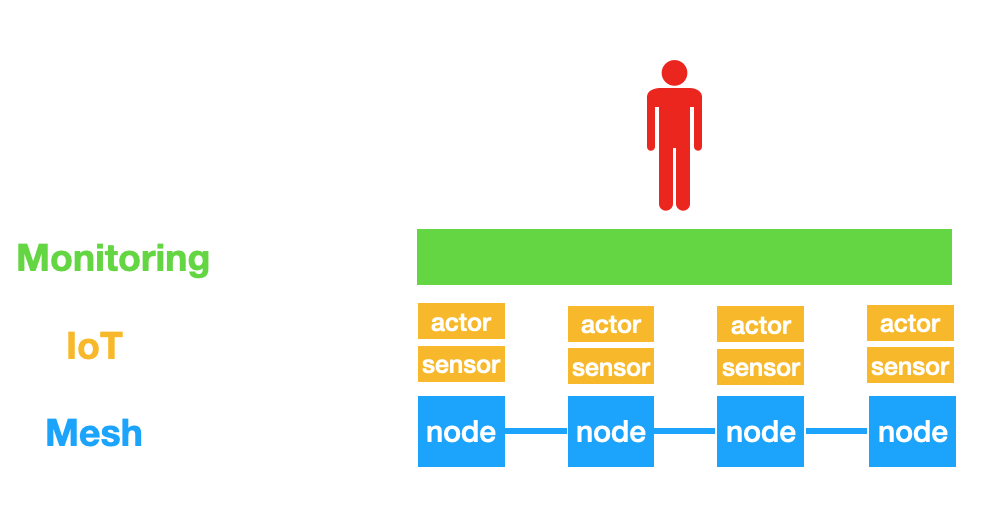
\includegraphics[scale=0.31]{images/structure.png}
            \caption{Struktur (Quelle: eigene Darstellung)}
        \end{center}
    \end{figure}
\end{abstract}

\begin{otherlanguage}{english}
\begin{abstract}
	
	At a school, classrooms are the most important place for the performance of pupils, the conditions in these classrooms should be optimal for learning success, in reality there are often shortcomings (e.g. low-oxygen air) that could easily be remedied. It is therefore advantageous to be able to record the conditions in the individual classrooms in order to take measures (open the window) on the one hand, and to obtain evaluable information for the heating mode (temperature) on the other.

	A mesh network should therefore make it possible to connect the sensors and actuators distributed throughout the HTL-Leonding building.

	The use of a mesh network enables simple integration of additional sensors and actuators, and the school network is not used.

	As part of this work, the mesh infrastructure was initially created (hardware configuration and software integration of nodes into the mesh network), and an IoT network was implemented as an application, which enables communication between the individual components using a message broker. The visualization, as a third component, can represent the current state of the IoT network and answer following questions : Which components (nodes) are online, which messages (e.g. temperature values) are transmitted, etc.

	\begin{figure}[H]
        \begin{center}
            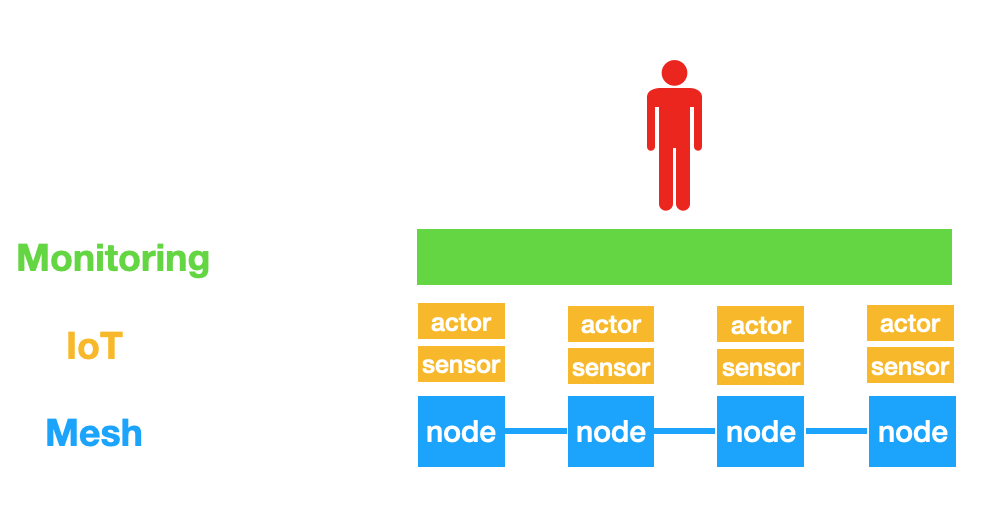
\includegraphics[scale=0.31]{images/structure.png}
            \caption{Structure (source: own source)}
        \end{center}
    \end{figure}
\end{abstract}
\end{otherlanguage}


\section*{Autoren der Diplomarbeit}
\subsection*{Tim Untersberger}
\subsubsection*{Aufgabenbereich}
% TODO: write
\begin{figure}[H]
	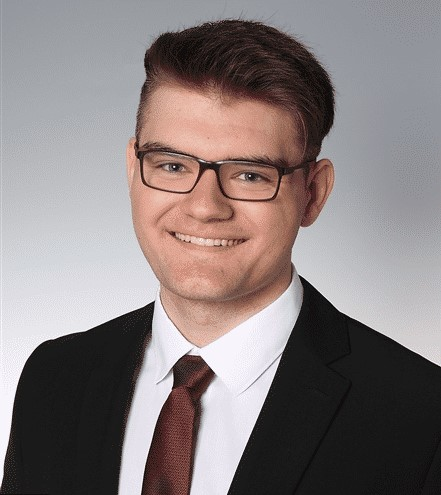
\includegraphics[scale=0.3]{images/tim_untersberger.jpg}
\end{figure}
\begin{table}[htb]
\begin{tabular}{ll}
Name:                            & Tim Untersberger          \\
Geburtsdatum:                    & 15. April 2001                   \\
E-Mail:                          & timuntersberger2@gmail.com          \\
                                 &                               \\
\textbf{Bildungsweg:}            &                               \\  
2007 bis 2011                    & Volksschule Doppl          \\
2011 bis 2015                    & NMS Hart     \\
seit 2015                        & HTL Leonding, Informatik      \\
                                 &                               \\
\textbf{Berufliche Erfahrung:}   &                               \\
Sommer 2016                      & {Colour \& Point}, Softwareentwickler \\
Sommer 2018                      & Runtastic, Softwareentwickler \\
                                 &                               \\
\textbf{Sprachliche Kenntnisse:} &                               \\
Deutsch                          & Muttersprache                 \\
Englisch                         & Fließend                     
\end{tabular}
\caption{Tim Untersberger}
\end{table}
\pagebreak
\subsection*{Stefan Waldl}
\subsubsection*{Aufgabenbereich}
\begin{figure}[H]
	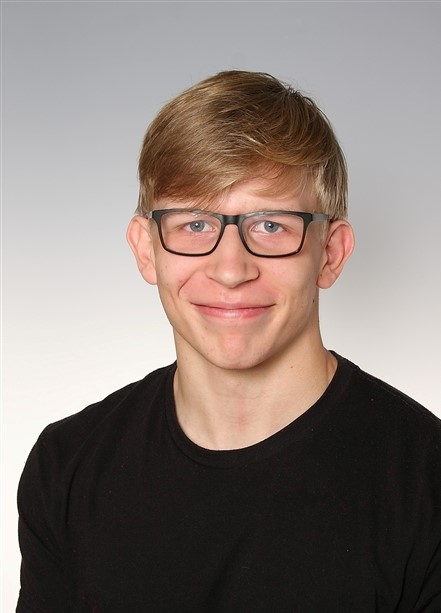
\includegraphics[scale=1]{images/stefan_waldl.jpg}
\end{figure}
\begin{table}[htb]
\begin{tabular}{ll}
Name:                            & Stefan Waldl          		 \\
Geburtsdatum:                    & 26. März 2000                 \\
E-Mail:                          & waldl.stefan@gmail.com        \\
                                 &                               \\
\textbf{Bildungsweg:}            &                               \\  
2006 bis 2010                    & Volksschule 28      		     \\
2010 bis 2015                    & BRG Ramsauerstraße    	 	 \\
seit 2015                        & HTL Leonding, Informatik      \\
                                 &                               \\
\textbf{Berufliche Erfahrung:}   &                               \\
Sommer 2017                      & CBCX-Betting Technologies, Softwareentwickler \\
Sommer 2018                      & CBCX-Betting Technologies, Softwareentwickler \\
                                 &                               \\
\textbf{Sprachliche Kenntnisse:} &                               \\
Deutsch                          & Muttersprache                 \\
Englisch                         & Fließend                     
\end{tabular}
\caption{Stefan Waldl}
\end{table}
\pagebreak
 

\section*{Danksagung}

An dieser Stelle möchten wir uns bei all denjenigen bedanken, die uns während der Planung und Durchführung dieser Diplomarbeit unterstützt und motiviert haben.

Ganz besonderen Dank an Herrn Prof. Thomas Stütz und Herrn Prof. Gerald Köck, welche uns bereits sehr früh unterstützt und unser Augenmerk auf die richtigen Technologien gelenkt haben, sowie uns auch betreut und unsere Arbeit begutachtet haben.

Bedanken wollen wir uns auch bei all unseren KorrekturleserInnen der Dokumente, welche uns für eine fehlerfreie und ordentliche Einreichung beiseite standen. % Declaration of Academic Honesty, Abstracts, Acknowledgments, 

\tableofcontents

\chapter{Ausgangssituation und Zielsetzung}

\section{Ausgangssituation}
Die HTBLA-Leonding ist eine BHS im Raum Oberösterreich, welche für ihre gute Ausbildung und interessanten Projekte im Bereich der Informationstechnologie bekannt ist.

\section{Beschreibung des Problembereichs}
In den Klassenräumen fehlt es oft an Sauerstoff, manchmal ist auch die Temperatur nicht adäquat. Dieseh kann eine Reihe von unerwünschten Symptomen hervorrufen, wie zum Beispiel: 

\begin{itemize}
    \item Kopfschmerzen
    \item Ermüdung
    \item Schwindel
    \item Übelkeit
    \item mehr Probleme mit Asthma und Allergien
\end{itemize}

Die oben gennannten Symptome sind in einer Umgebung wie der Schule unbedingt zu vermeiden, da es ansonsten zu einem Konzentrationsverlust der Schüler führt.

Um zusätzlich eine Regelung der Heizung vornehmen zu können sind weitere Informationen der einzelnen Klassenräume, wie die Temperatur, notwendig. Weiters wird es rund um die Uhr ermöglicht,  geöffnete Fenster zu lokalisieren und mit dieser Information Schäden an der Schule zu verhindern.

\section{Aufgabenstellung}
%todo
drei Ebenen
nodes senden Nachrichten
ota
systemarchitektur
dann einzelne Komponente

\begin{figure}[H]
    \centering
    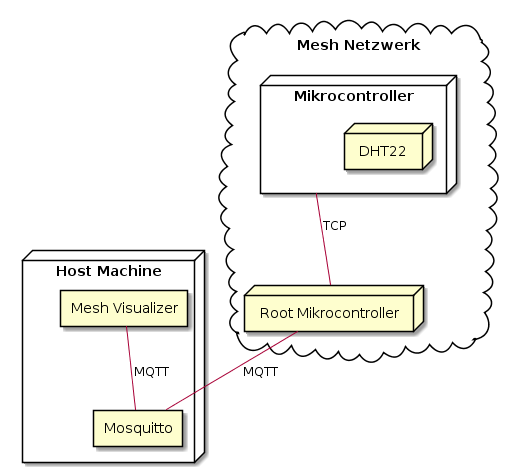
\includegraphics[scale=0.8]{diagrams/deployment.png}
    \caption{Systemarchitektur (Quelle: Eigene Darstellung)}
    \label{abb:deployment}
\end{figure}

Um die Sensoren in der Schule platzieren zu können, ist es erforderlich, zuerst eine Infrastruktur für die Auswertung der Sensoren zu gestalten.

\section{Zielbestimmung}
Unterricht findet in einer Lernumgebung statt
Schüler lernen

Die Knoten eines Mesh-Netzwerks können gegenseitig Nachrichten versenden und reagieren automatisch auf ausfallende Knoten.
\chapter{AufgabenStellung}
\chapter{Verwendete Technologien}\label{cha:used-technologies}

\section{Message Queuing Telemetry Transport (MQTT)}\label{sec:mqtt}

Im Laufe der Arbeit werden folgende Begriffe erwähnt, welche hier erklärt werden:

\begin{enumerate}
    \item \textbf{Broker}:
    
    Ein Server, der alle Nachrichten von den Clients empfängt und diese dann an die entsprechenden Zielclients weiterleitet.

    \item \textbf{Topic}:
    
    In MQTT verweist das Wort Topic auf eine UTF-8-Zeichenfolge, die der Broker zum Filtern von Nachrichten für jeden verbundenen Client verwendet. Das Topic besteht aus einer oder mehreren Topiclevels. Jedes Topiclevel ist durch einen Slash getrennt.
    
    \item \textbf{Message}:
    
    Eine MQTT Message ist ein beliebiges Array von Bytes, welche an ein bestimmtes Topic gesendet werden.

    Wenn in dem Kapitel \ref{sec:own-libraries-mqtt} von einer MQTT Message geschrieben wird, dann steht dies für die Struktur, welche in der selben Library definiert wird.

    \item \textbf{Quality of Service (QoS)}:
    
    Das Quality of Service (QoS) Level ist eine Vereinbarung zwischen dem Absender einer Nachricht und dem Empfänger einer Nachricht, die die Zustellgarantie für eine bestimmte Nachricht definiert.
\end{enumerate}

\subsection{QoS}\label{sec:mqtt-qos}

In der nachstehenden Aufzählung werden die drei verschiedenen Arten von QoS näher erläutert, welche von der HiveMq Website\cite{hivemq} zusammengefasst wurden.

\begin{enumerate}
    \item \textbf{QoS 0 - maximal einmal}:
    Die minimale QoS-Stufe ist 0. Dieser Service-Level garantiert eine bestmögliche Lieferung. Es gibt keine Liefergarantie. Der Empfänger bestätigt den Empfang der Nachricht nicht und die Nachricht wird vom Absender nicht gespeichert und erneut gesendet. QoS-Stufe 0 wird oft als "fire and forget" bezeichnet und bietet die gleiche Garantie wie das zugrunde liegende TCP-Protokoll. 

    \begin{figure}[H]
        \begin{center}
            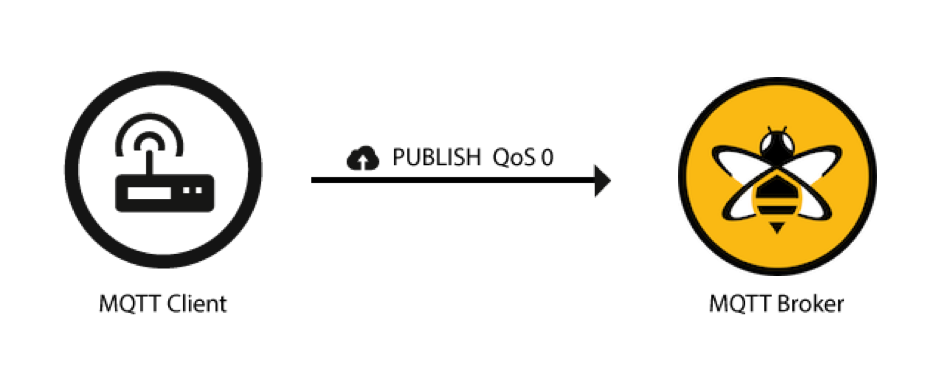
\includegraphics[scale=0.8]{images/QoS-0.png}
            \caption{MQTT QoS 0 \cite{hivemq}}
        \end{center}
    \end{figure}

    \item \textbf{QoS 1 - mindestens einmal}:
    
    QoS Level 1 garantiert, dass eine Nachricht mindestens einmal an den Empfänger übermittelt wird. Der Absender speichert die Nachricht, bis er vom Empfänger ein Rückmeldung erhält, das den Empfang der Nachricht bestätigt. Es ist möglich, dass eine Nachricht mehrmals gesendet oder zugestellt wird.

    \begin{figure}[H]
        \begin{center}
            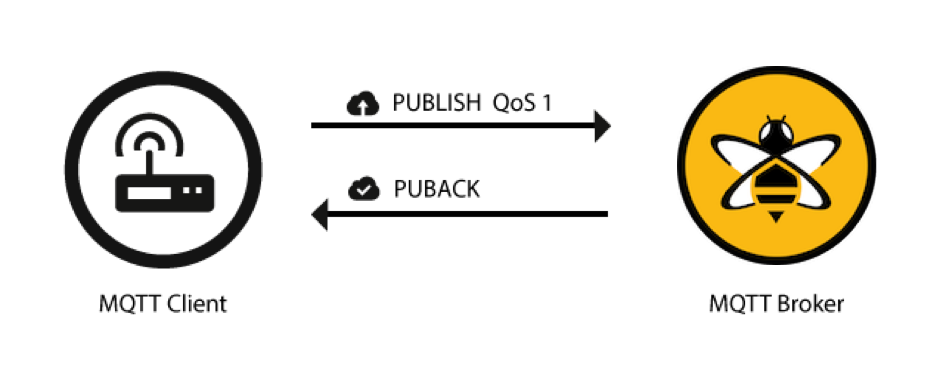
\includegraphics[scale=0.8]{images/QoS-1.png}
            \caption{MQTT QoS 1 \cite{hivemq}}
        \end{center}
    \end{figure}

    \item \textbf{QoS 2 - genau einmal}:
    
    QoS 2 ist das höchste Servicelevel in MQTT. Diese Stufe garantiert, dass jede Nachricht nur einmal von den vorgesehenen Empfängern empfangen wird. QoS 2 ist die sicherste und langsamste Servicequalität. Die Garantie wird durch mindestens zwei request/response flows zwischen dem Sender und dem Empfänger bereitgestellt. 

    \begin{figure}[H]
        \begin{center}
            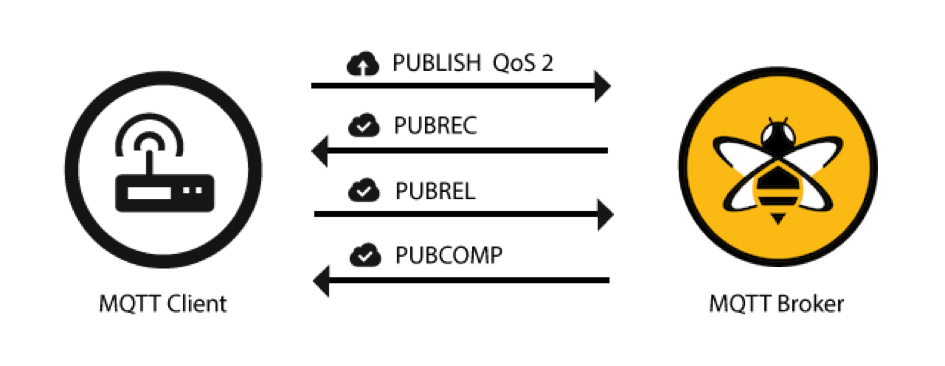
\includegraphics[scale=0.8]{images/QoS-2.png}
            \caption{MQTT QoS 2 \cite{hivemq}}
        \end{center}
    \end{figure}
\end{enumerate}

\section{ESP-IDF Toolchain}\label{sec:esp-idf-toolchain}
Um die Toolchain verwenden zu können muss man sich in einem ESP-IDF Projektverzeichnis befinden. Hier kann ist es möglich, mit folgendem Befehl, den ESP zu konfigurieren:

\begin{verbatim}
    idf.py menuconfig
\end{verbatim}

Dieser Befehl sollte zu folgendem Menü führen:
\begin{figure}[H]
    \begin{center}
        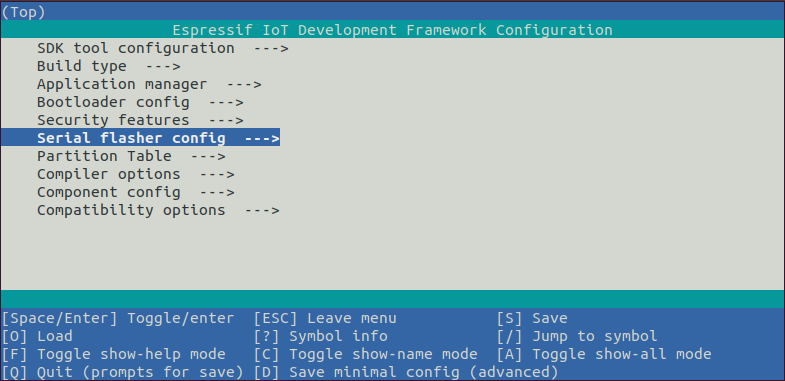
\includegraphics[scale=0.5]{images/menuconfig.png}
        \caption{menuconfig \cite{menuconfig_picture}}
    \end{center}
\end{figure}
Dieses Menü wird verwendet um Projekt spezifische Variablen zu setzten. Wie zum Beispiel:
\begin{itemize}
    \item Netzwerkname
    \item Netzwerkpasswort
    \item Takt des Prozessors
    \item Parition Table Variante
    \item \dots und viele mehr
\end{itemize}

\subsection{KConfig.projbuild}\label{sec:esp-idf-projbuild}
Sind die, von Espressif, zur Verfügung gestellten Menüs nicht genug, so ist es möglich eine \textbf{KConfig.projbuild} Datei anzulegen. Mit dieser Datei ist es möglich neue Top-Level Menüeinträge und Untermenüeinträge zu generieren. Dies wird benötigt, da in der standarmäßigen \textbf{menuconfig} nur der Großteil der gebrauchten Konfigurations-Felder zur Verfügung gestellt werden.

\subsection{Kompilieren}
Damit die fertigen Espressif Beispiele auf einem Dual-Core ESP funktionieren, muss sich dieser im Single-Core Modus befinden.

Ist das Projekt richtig konfiguriert kann es mit folgendem Befehl gebuildet werden:
\begin{verbatim}
    idf.py build
\end{verbatim}

Mit diesem Befehl wird die Anwendung kompiliert sowie der Bootloader und der Partition Table erstellt.

Sollten beim Kompilieren Fehler auftreten, so werden diese in der Konsole ausgegeben.

\subsection{Flashen}
Verläuft das Kompilieren Fehlerfrei, kann das Programm mit diesem Befehl auf den ESP geflasht werden:
\begin{verbatim}
    idf.py flash
\end{verbatim}

Sollte es ein Problem beim Flashen geben, liegt dies häufig an einem kaputten USB-Kabel.

Zumeist ist ein Problem beim Flashen auf ein kaputtes USB-Kabel zurückzuführen.

\subsubsection{IDF Monitor}\label{sec:monitor}
Der IDF-Monitor ist ein serielles Terminalprogramm, das serielle Daten zum und vom seriellen Anschluss des Zielgeräts weiterleitet.

Ist das Programm bereits auf dem ESP kann es mit folgendem Befehl auf dem IDF Monitor, überprüft werden.

\begin{verbatim}
    idf.py monitor
\end{verbatim}

Mit dem nachstehenden Befehl kann das Programm gebuildet, geflasht und upgeloadet werden. Dies erspart den Aufwand jeden Befehl einzeln einzugeben.

\begin{verbatim}
    idf.py flash monitor
\end{verbatim}

\section{Nodejs}\label{sec:nodejs}

Nodejs ist eine Laufzeit die auf der Javascript Engine von Chrome aufbaut. Nodejs wurde für das Backend des OTA Servers verwendet.

\subsection{Warum Nodejs?}

Bei der Überlegung welche Sprache bzw. welches Framework für das backend gewählt wird, war die Entscheidung sehr leicht.
Die Anforderungen des OTA Servers sind sehr einfach. Der Server dient nur zur Bereitstellung der Firmwares und beschreibende Informationen über die Firmwares selber.
Da dies nicht CPU intensiv ist sondern I/O intensiv, wurde in diesem Fall Nodejs gewählt.

\subsection{Event Loop}

\subsubsection{Was ist der Event Loop?}

Nodejs selber ist single-threaded deswegen ist der Event Loop einer der wichtigsten Bestandteile von Nodejs.
Der Event Loop erlaubt es nicht-blockenede I/O Operationen durchzuführen. Dies passiert durch die Abladung auf den Kernel von so vielen Operationen wie möglich.
\newline
\newline
Die meisten modernen Kernels sind multi-threaded. Das bedeutet, dass sie mehrere Operationen im Hintergrund unterstützen.

\subsubsection{Wie funktioniert der Event Loop?}

\begin{figure}[H]
    \begin{center}
        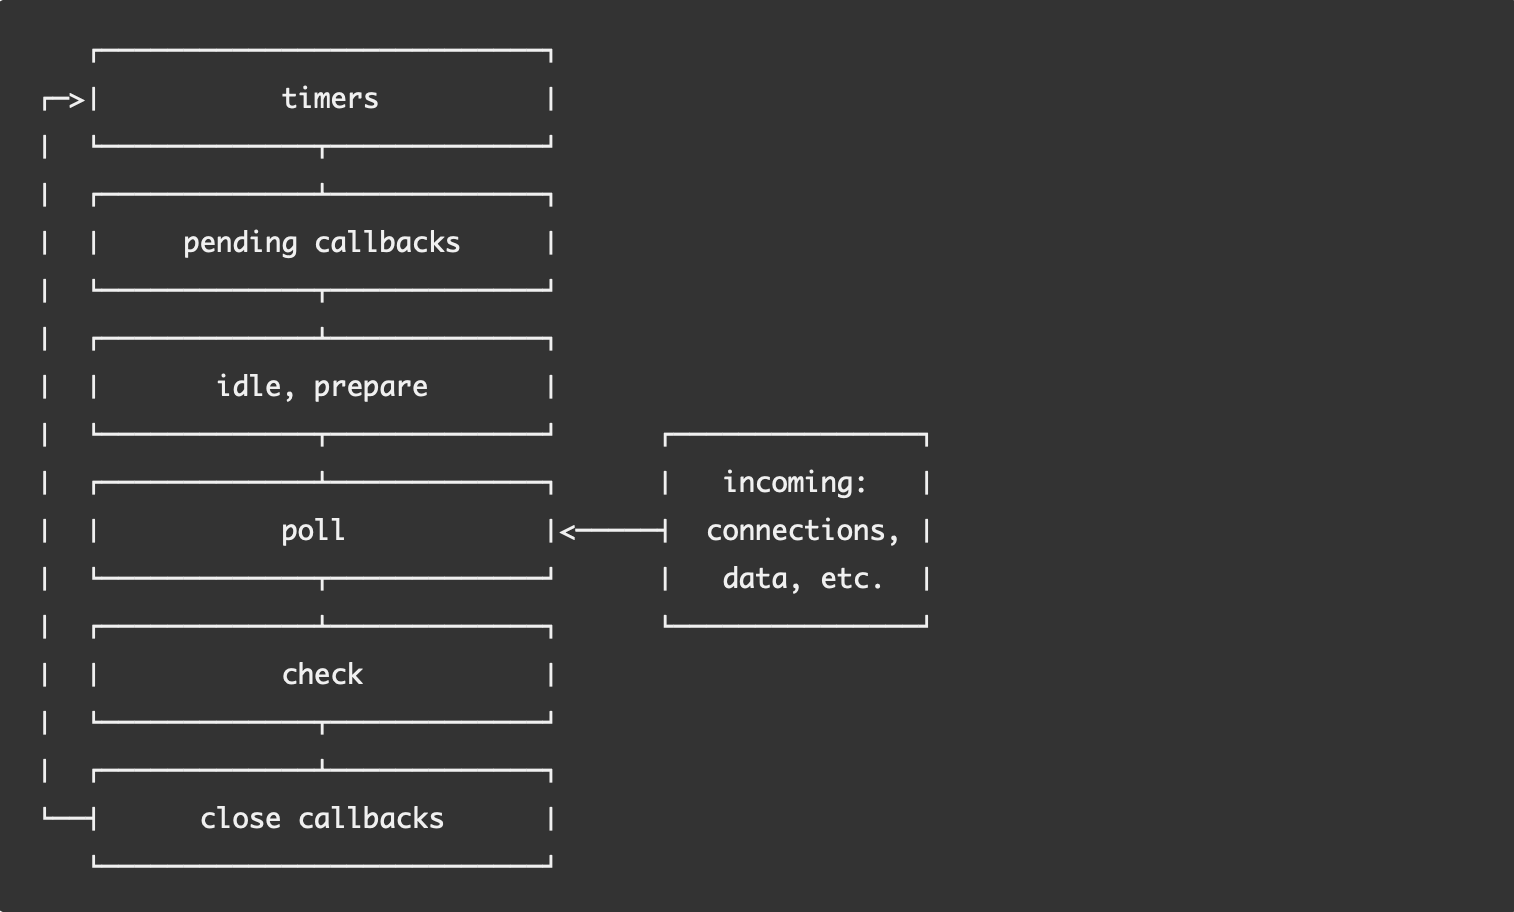
\includegraphics[scale=0.5]{images/nodejs_event_loop.png}
        \caption{Nodejs Event Loop \cite{nodejs_event_loop}}
    \end{center}
\end{figure}

Jeder Block im obigen Bild wird als Phase bezeichnet.
Jede Phase verfügt über eine First-In-First-Out-Warteschlange (FIFO-Warteschlange) mit auszuführenden Rückrufen. 
Während jede Phase auf ihre Weise etwas Besonderes ist, führt sie im Allgemeinen,
wenn die Ereignisschleife in eine bestimmte Phase eintritt, alle für diese Phase spezifischen Operationen aus und führt dann Rückrufe in der Warteschlange dieser Phase aus, 
bis die Warteschlange erschöpft ist oder die maximale Anzahl von Rückrufen ausgeführt hat. 
Wenn die Warteschlange erschöpft ist oder das Rückruflimit erreicht ist, wechselt die Ereignisschleife zur nächsten Phase und so weiter.
\newline
\newline
Da für jeden dieser Vorgänge möglicherweise mehr Vorgänge geplant werden und neue Ereignisse, 
die in der Abfragephase verarbeitet wurden, vom Kernel in die Warteschlange gestellt werden, 
können Abrufereignisse in die Warteschlange gestellt werden, während Abrufereignisse verarbeitet werden. 
Infolgedessen können lange laufende Rückrufe dazu führen, dass die Abfragephase viel länger als der Schwellenwert eines Timers läuft. 

\subsubsection{Phasen}

\begin{itemize}
    \item \textbf{timers:} In dieser Phase werden von setTimeout () und setInterval () geplante Rückrufe ausgeführt.
    \item \textbf{pending callbacks:} führt I/O Callbacks aus, die auf die nächste Iteration verschoben werden
    \item \textbf{idle, prepare:} wird nur intern verwendet
    \item \textbf{poll:} neue I/O Events abrufen; I/O bezogene Callbacks ausführen (fast alle mit Ausnahme von schließ Callbacks, die von Timers geplant werden, und setImmediate ()); Der Knoten wird hier gegebenenfalls blockiert
    \item \textbf{check:} setImmediate() Callbacks werden hier ausgeführt
    \item \textbf{close callbacks:} schließ Callbacks werden ausgeführt
\end{itemize}

Zwischen jedem Durchlauf des Event Loops prüft Nodejs, ob es auf asynchrone I/O oder Timer wartet, und fährt sauber herunter, wenn keine vorhanden sind.

\cite[Zitiert von der offizielen Nodejs Website]{nodejs_event_loop_how_does_it_work}

\section{Platform IO}\label{sec:platformio}

PlatformIO ist ein fortschrittliches und äußerst vielseitiges Ökosystem für die IoT-Entwicklung, das eine IDE, ein Build-System, einen Unified Debugger und einen Bibliotheksmanager umfasst. Es bietet Unterstützung für mehr als 550 Entwicklungsboards, mehr als 25 Entwicklungsplattformen und mehr als 10 nützliche Frameworks. Die PlatformIO IDE ist ein plattformübergreifendes Dienstprogramm für die schnelle berufliche Weiterentwicklung mit integriertem C / C++ - Intelligent Code Completion, Smart Code Linter und erweitertem Serial Port Monitor. PlatformIO kann auch in die gängigen IDEs und kontinuierlichen Integrationssysteme integriert werden, um die Zeit für die Bereitstellung von IoT-Anwendungen zu verkürzen.\cite{platformio_about_us}

PlatformIO ist in reinem Python geschrieben und hängt nicht von zusätzlichen Bibliotheken / Tools eines Betriebssystems ab. So kann man mit PlatformIO auf Windows, Macintosh und Linux arbeiten.

\section{Docker}\label{sec:docker}

Docker ist ein Open-Source-Projekt zur Automatisierung der Bereitstellung von Anwendungen als tragbare Container, die überall ausgeführt werden können. 

\subsection{Docker vs. Virtuelle Maschinen}\label{sec:docker-vm}

\subsubsection{Virtuelle Maschinen}

\begin{figure}[H]
    \begin{center}
        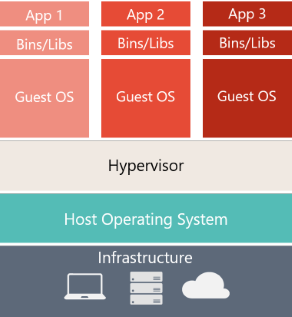
\includegraphics[scale=0.8]{images/docker-vm.png}
        \caption{Docker Virtuelle Maschine (Quelle: eigene Darstellung)}
    \end{center}
\end{figure}

Zu den virtuellen Maschinen gehören die Anwendung, die erforderlichen Bibliotheken oder Binärdateien sowie ein vollständiges Gastbetriebssystem. Die vollständige Virtualisierung erfordert mehr Ressourcen als die Containerisierung. \cite{docker}

\subsubsection{Docker}

\begin{figure}[H]
    \begin{center}
        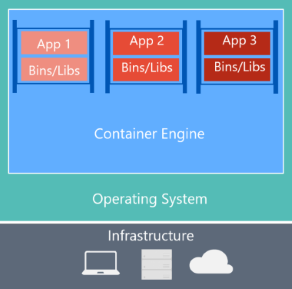
\includegraphics[scale=0.8]{images/docker.png}
        \caption{Docker (Quelle: eigene Darstellung)}
    \end{center}
\end{figure}

Container enthalten die Anwendung und alle ihre Abhängigkeiten. Sie teilen den Betriebssystemkern jedoch mit anderen Containern und werden als isolierte Prozesse im Benutzerbereich des Host-Betriebssystems ausgeführt. (Außer in Hyper-V-Containern, in denen jeder Container innerhalb einer speziellen virtuellen Maschine pro Container ausgeführt wird.) \cite{docker}

\subsection{Begriffe}\label{docker-terminology}

Im Laufe der Arbeit werden folgende Begriffe erwähnt:

\begin{enumerate}
    \item \textbf{Container}:
    
    Ein Container ist eine Instanz eines Images. Er repräsentiert die Ausführung einer einzelnen Anwendung, eines Prozesses oder eines Dienstes. 

    \item \textbf{Image}:
    
    Ein Image ist ein Paket mit allen Abhängigkeiten und Informationen, die zum Erstellen eines Containers erforderlich sind. Ein Image enthält alle Abhängigkeiten (z. B. Frameworks) sowie die Bereitstellungs- und Ausführungskonfiguration, die von einer Container-Laufzeit verwendet werden soll. 

    \item \textbf{Volume}:
    
    Ein Volume ist ein beschreibbares Dateisystem, das der Container verwenden kann. Da Images schreibgeschützt sind fügen Volumes eine beschreibbare Ebene über dem Image hinzu, sodass die Programme Zugriff auf ein beschreibbares Dateisystem haben. 

    \item \textbf{Network}:

    In einem Docker Network können Container auf sich gegenseitig mittels ihren Namen referenziern. Dies erleichtert das miteinander Arbeiten von verschiedenen Containern.
\end{enumerate}

\section{Docker Compose}\label{sec:docker-compose}

Docker-compose ist ein Tool zum Definieren und Ausführen von Docker-Anwendungen mit mehreren Containern. Mit Compose wird eine YAML-Datei verwendet, um die Dienste von Anwendung zu konfigurieren. Anschließend werden alle Dienste mit einem einzigen Befehl erstellt und gestartet. \cite{docker_compose_description}

\subsection{Docker Compose Beispiel}

\begin{figure}[H]
    \begin{center}
        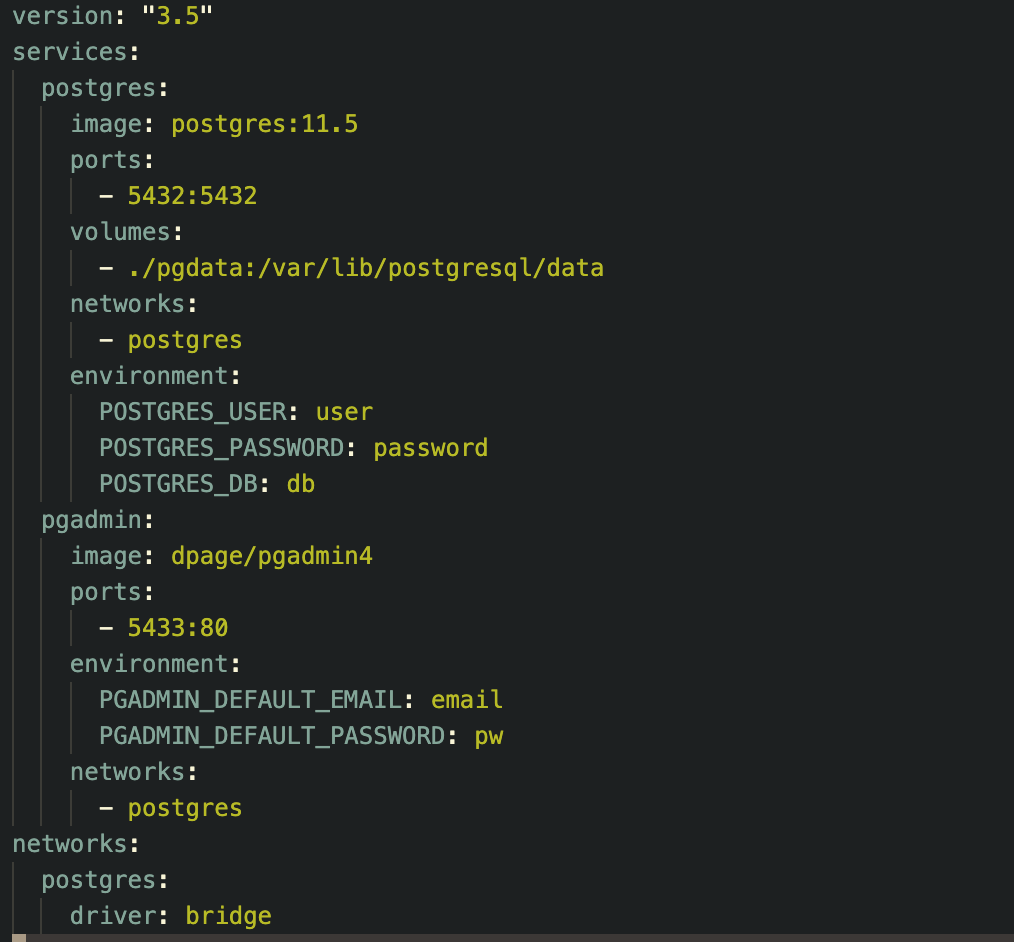
\includegraphics[scale=0.8]{images/docker_compose_example.png}
        \caption{Docker Compose Beispiel (Quelle: eigene Darstellung)}
        \label{abb:docker-compose-example}
    \end{center}
\end{figure}

In der obigen Abbildung kann man das docker-compose.yml file von dem OTA Server sehen.

Die Struktur eines docker-compose files ist im Normalfall immer gleich. Am Anfang definiert man welche Version des Standards man verwendet und anschließend die verschiedenen Dienste. Der OTA Server benötigt nur 2 Dienste:

\begin{enumerate}
    \item Postgres
    \item PgAdmin4
\end{enumerate}

In Abbildung \ref{abb:docker-compse-example} wird ein Netzwerk explizit erstellt. Es ist auch möglich das Netwerk implizit zu erstellen, indem man den networks Bereich von ganz unten entfernt.

\subsubsection{Postgres}

Datenbank für die Speicherung von den Informationen über die verschieden Firmwares die gerade auf dem Server hochgeladen sind.

Die Datenbank braucht irgendeinen Weg um mit der Außenwelt kommunizieren zu können, deswegen wird der interne Port 5432 auf den externen Port 5432 geleitet.

Damit die Absicherung der Datenbank leicht verläuft wird ein Volume für die Datenbank erstellt, worin sich die Daten der Datenbank befinden. In dieser docker-compose Datei wird das Volume implizit erstellt. 

Man kann es auch explizit erstellen wie folgt:

\begin{verbatim}
    volumes:
        pgdata:
\end{verbatim}

Mit den Umgebungsvariablen kann man die Standardwerte überschreiben. Die Datenbank hat in der obigen Abbildung den Benutzer \textit{user} mit dem Passwort \textit{password} und der default Datenbank \textit{db}.

\subsubsection{PgAdmin4}

PgAdmin4 ist eine web-basierte Benutzeroberfläche für Postgres.

Sie ist die PhpMyAdmin Oberfläche in der postgres Welt.

Die Software binded automatisch auf den Port 80, was für Entwicklungszwecke sehr unpraktisch ist, da Port 80 auf Ubuntu zum Beispiel Adminrechte benötigt. Deswegen wird der interne Port 80 auf den externen Port 5433 umgeleitet.

Mit den Umgebungsvariablen \textit{PGADMIN\_DEFAULT\_EMAIL} und 
\textit{PGADMIN\_DEFAULT\_PASSWORD} werden die default Logindaten für PgAdmin4 definiert. 
\pagebreak

\section{Utility lib Köck}\label{sec:utility-lib-koeck}
Dies ist Professor Köcks Library Sammlung, welche er persönlich verfasste. Sämtliche Technologien, welche durch die Libraries untersützt werden, sind in folgender Abbildung zu sehen.

\begin{figure}[H]
    \begin{center}
        \includegraphics[scale=0.9]{images/utility_lib_köck_own.PNG}
        \caption{Technologien Utility lib (Quelle: eigene Darstellung)}
    \end{center}
\end{figure}

\pagebreak
Dazu sind folgende Sensor Libraries ebenfalls enthalten:

\begin{figure}[H]
    \begin{center}
        \includegraphics[scale=0.9]{images/utility_lib_köck_sensors.PNG}
        \caption{Sensoren und Aktoren Utility lib (Quelle: eigene Darstellung)}
    \end{center}
\end{figure}

Im Laufe der Arbeit erfolgte ein Umstieg auf die offiziellen Espressif Libraries, da Professor Köcks Library Sammlung aufgrund fehlender Funktionalität für diese Diplomarbeit nicht mehr geeignet war.

Da alle Espressif Libraries in der Programmiersprache C geschrieben sind, ist es nicht möglich diese mit den Libraries von Professor Köck gleichzeitig zu verwenden. Da diese in C++ geschrieben sind und die Espressif Libraries Funktionen aus C verwenden, welche in C++ nicht unterstützt werden. Um Kompatibilität herzustellen ist es bei jeder Anwendung notwendig die Espressif Libraries anzupassen.
\chapter{Ausgewählte Aspekte}

\section{Verwendete Hardware}

\subsection{DHT22}

\begin{figure}[H]
    \begin{center}
        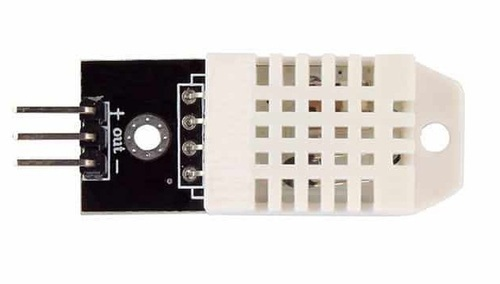
\includegraphics[scale=1]{images/dht22.png}
        \caption{Bild DHT22 \cite{dht22_picture}}
    \end{center}    
\end{figure}



Der DHT22, oder auch AM2302, ist ein digitaler Temperatur und Feuchtigkeissensor, welcher ein digitales Signal der Sensordaten über den Daten-Pin ausgibt. Jedes Exemplar dieses Sensor Modells wurde in einer Kalibriekammer kalibriert. Dieser Kalibrierkoeffizient wird dann im am Bord one time programmable Speicher (OTP Memory \ref{sec:otp}) gespeichert.
\pagebreak

Die Technischen Daten des Sensors sind:
\begin{figure}[H]
    \begin{center}
        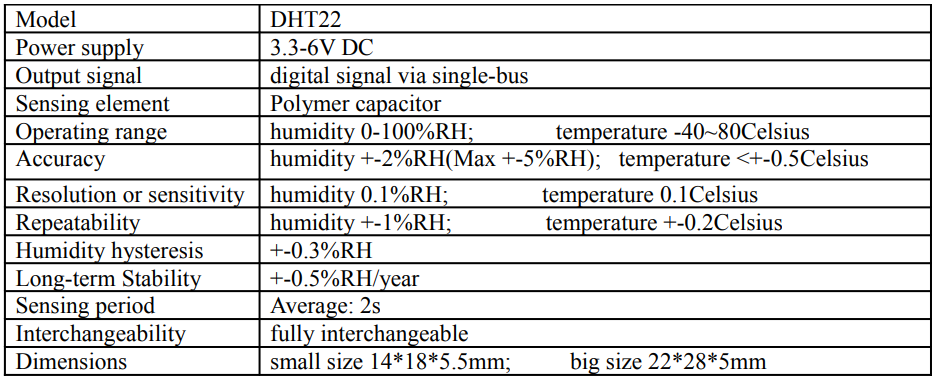
\includegraphics[scale=0.6]{images/dht22_datasheet.png}
        \caption{Daten Dht22 \cite{dht22_datasheet_sparkfun}}
    \end{center}
\end{figure}

Zu den Vorteilen des DHT22 zählen:
\begin{itemize}
    \item Kleiner Formfaktor (15,1mm x 25,1mm x 7,7mm)
    \begin{figure}[H]
        \begin{center}
            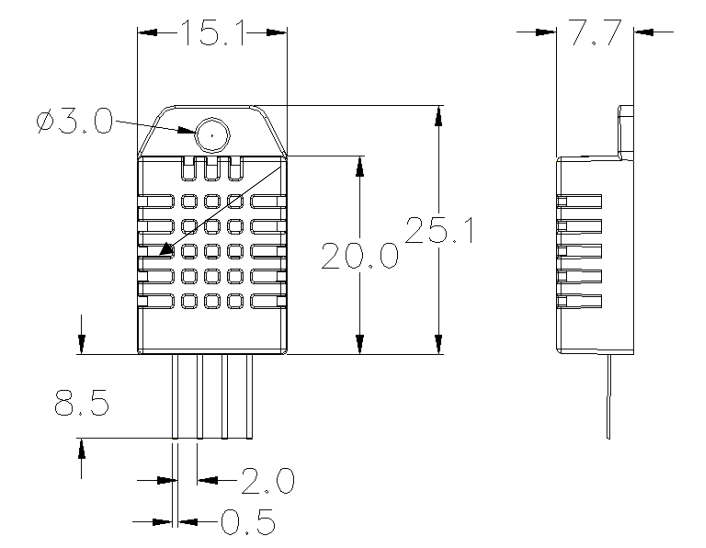
\includegraphics[scale=0.6]{images/dht22_formfaktor.png}
            \caption{Formfaktor Dht22 \cite{dht22_datasheet_sparkfun}}
        \end{center}
    \end{figure}
    \item Niedriger Stromverbrauch (3,3-6 Volt)
    \item Lange Übertragunsdistanz (20 Meter)
\end{itemize}

Der Nachteil des Sensors ist:
\begin{itemize}
    \item Wartezeit zwischen neuen Sensordaten (mindestens 2 Sekunden)
\end{itemize}

\subsubsection{OTP Memory}\label{sec:otp}
OTP Speicher ist eine spezielle Form von nicht flüchtigem Speicher, der es genau ein Mal erlaubt auf den Speicher zu schreiben. Wenn der Speicher einmal programmiert ist behält er seine Informationen für immer, auch über Stromverlust.

Beispiele dafür sind:
\begin{itemize}
    \item Boot code
    \item Encryption keys
    \item Konfigurationsparameter für analoge Sensoren
\end{itemize}

\subsection{NodeMCU ESP32}

\begin{figure}[H]
    \begin{center}
        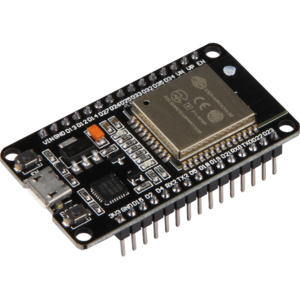
\includegraphics[scale=0.8]{images/NodeMCU-ESP32.png}
        \caption{Bild NodeMCU ESP32 \cite{nodemcu_picture_joy-it}}
    \end{center}
\end{figure}

Das NodeMCU ESP32 ist ein prototyping Board. Die wichtigste Komponente dieses ESPs ist das ESP-WROOM-32 \ref{sec:esp-wroom-32}, es stell das Gehirn dieses Mikrocontrollers dar.

\subsubsection{ESP-WROOM-32}\label{sec:esp-wroom-32}

Das ESP-WROOM-32 ist ein generisches MCU Modul mit integriertem Wi-Fi, Bluetooth und Bluetooth low energy. So ermöglicht einem dieses Modul sich beispielsweise mit Wlan-Router oder einem Handy zu verbinden. Weiters ist es durch den niedrigen Schlafstrom von 5 µA gut für den Bateriebetrieb geeignet.

\begin{figure}[H]
    \begin{center}
        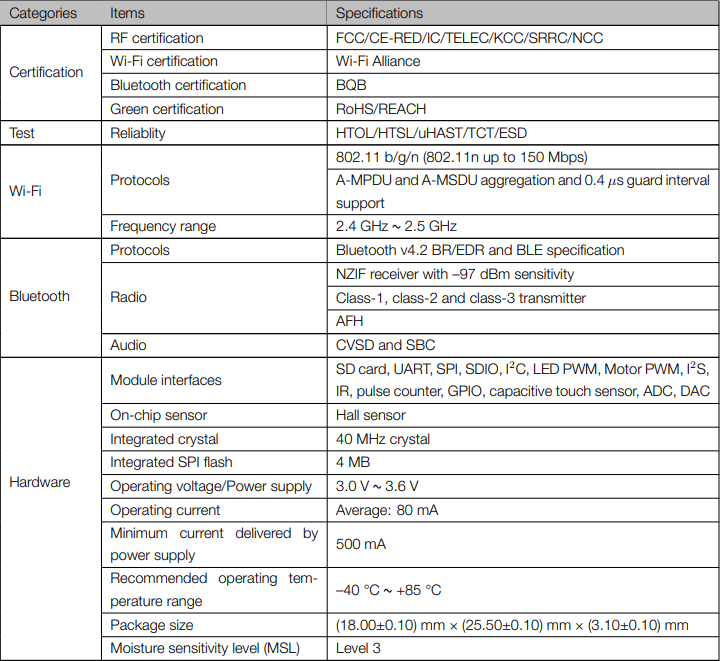
\includegraphics[scale=0.78]{images/esp32-wroom-32.png}
        \caption{ESP32-WROOM-32 Spezifikationen\cite{esp32-wroom-32_secifications}}
    \end{center}
\end{figure}

\section{Over The Air Update (OTA)}\label{sec:ota}

\subsection*{Problemstellung}\label{sec:problem}
Mikrocontroller befinden sich, wenn sie sich in einem laufendem System befinden meist an ungünstigen Orten, an die man nur mit hohem Aufwand gelangt.
Bis jetzt musste man den Computer physisch mit einem Kabel mit dem Mikrocontroller verbinden um neue Firmware auf den Kontroller zu spielen.
OTA ermöglicht es den Mikrocontroller über das Netzwerk mit neuer Firmware zu versorgen, dabei muss der selektierte Microcomputer lediglich mit einem Wlan-Router verbunden sein und ein physisches Kabel wird überflüssig.

\subsection*{Wie OTA funktioniert}
Bei dem OTA-Vorgang wird zu aller erst die Config-Datei, des jeweiligen Mikrocontrollers, ausgelesen. In dierser Datei steht welche Firmware OTA herunterladen soll. Nun sendet der Mikrocontroller eine Anfrage mit dem, in der Config-Datei eingetragen, Namen der Firmware. Diese Anfrage dient dazu den Timestamp, an dem die Firmware das letzte Mal am Server geändert worden ist herauszufinden.\newline
Darauf antwortet der Server mit dem Timestamp.\newline
Nun überprüft der Mikrocontroller den Timestamp der letzten Änderung des Servers mit dem Timestamp der letzten Änderung der Firmware, die gerade installiert ist.\newline

Nun gibt es zwei Szenarien, die eintreten können:

\begin{itemize}
    \item Die Timestamps sind gleich. Das bedeutet, dass der Server und der Mikrocontroller beide die gleiche Firmware besitzen und es besteht kein Grund diese vom Server herunterzuladen.
    \begin{figure}[H]
        \begin{center}
            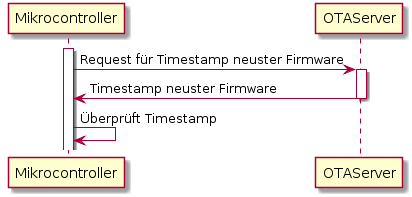
\includegraphics[scale=0.8]{diagrams/ota_sequence_same_timestamp.png}
            \caption{OTA Sequenz Timestamp gleich (Quelle: eigene Darstellung)}
        \end{center}
    \end{figure}
    \newpage
    \item Die Timstamps sind unterschiedlich. Das bedeutet, dass die Firmware am Server geändert wurde und der Mikrocontroller eine ältere Version besitzt.\newline
    Da davon ausgegangen wird, dass der Server immer die beste Version der Firmware bestitz, lädt der Mikrocontroller diese herunter und startet von der soeben heruntergeladenen Firmware neu.
    \begin{figure}[H]
        \begin{center}
            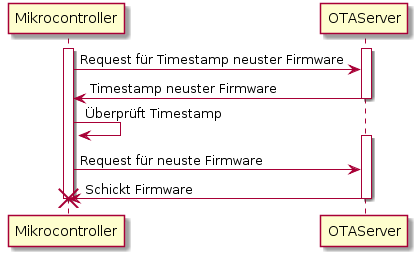
\includegraphics[scale=0.8]{diagrams/ota_sequence_different_timestamp.png}
            \caption{OTA Sequenz Timestamp anders (Quelle: eigene Darstellung)}
        \end{center}
    \end{figure}
\end{itemize}

% TODO: Deployment diagram.
\begin{figure}[H]
    \begin{center}
        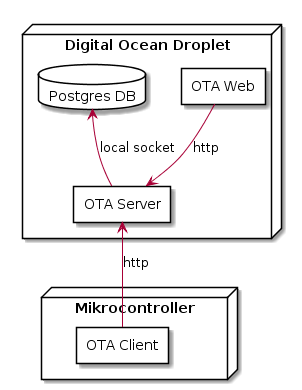
\includegraphics[scale=0.6]{diagrams/ota_deployment.png}
        \caption{OTA Deployment (Quelle: eigene Darstellung)}
    \end{center}
\end{figure}

\subsection{Partitions Tabelle}
Die Partitionstabelle ist bei OTA mitunter eines der wichtigsten Themen. Würde man diese Tabelle nicht richtig konfigurieren würde das Programm nicht einmal starten. Dazu kommt noch eine erschwerte Fehlersuche, da Errormeldungen bei der Arbeit mit Mikrocontrollern zu wünschen lassen.
Die Standard-Partitionstabelle ist je nach Hersteller anders. Um OTA zu ermöglichen ist es notwendig im Partitionstabelle mindestens eine, ausreichend große, OTA-Partition zu vergeben. Dabei ist es wichtig, dass diese Partition ausreichend Speicher für die gewünschte Firmware hat, da sonst der ganze Vorgang abgebrochen wird.

% TODO: Write about memory diagram
% TODO: Write about partition table diagram

\subsubsection{Übersicht}
Der Flash eines einzelnen ESP32 kann mehrere Apps sowie viele verschiedene Arten von Daten (Kalibrierungsdaten, Dateisysteme, Parameterspeicherung usw.) enthalten. Aus diesem Grund wird eine Partitionstabelle im Flash auf (Standardoffset) 0x8000 geflasht.

Die Länge der Partitionstabelle beträgt 0xC00 Byte (maximal 95 Partitionstabelleneinträge). Nach den Tabellendaten wird eine MD5-Prüfsumme angehängt, mit der die Integrität der Partitionstabelle überprüft wird. Wenn die Partitionstabelle aufgrund eines sicheren Starts signiert ist, wird die Signatur nach der Partitionstabelle angehängt.

Jeder Eintrag in der Partitionstabelle hat einen Namen (Bezeichnung), einen Typ (app, data, ota oder etwas anderes), einen SubType und den Offset im Flash, in dem die Partition geladen wird.

\subsubsection{Custom Partition Tables}
Bei komplexeren Anwendungen reichen die default Partitionstabellen nicht mehr aus und es muss eine angepasste Tabelle erstellt werden, welche aber auch genau auf die Bedürfnisse von gewissen Firmwares zugeschnitten werden kann.

Wenn die Option der Benutzerdefinierte Partitionstabelle ausgewählt wird. Muss manuel eine CSV-Datei erstellt werden, in der dann eine beliebige Anzahl von Partitionen mit folgenden Punkten eingetragen werden können:

\begin{itemize}
    \item Name
    \item SubType
    \item Offset
    \item Size
    \item Flags
\end{itemize}

\begin{figure}[H]
    \begin{center}
        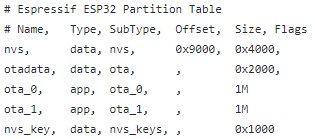
\includegraphics[scale=1]{images/partition_table.png}
        \caption{Beispiel Partitionstabelle (Quelle: eigene Darstellung)}
    \end{center}    
\end{figure}

\subsubsection{Name Feld}
Das Namensfeld kann beliebig gewählt werden. Es ist für den Mikrocontroller nicht von Bedeutung. Namen die länger als 16 Zeichen sind werden jedoch abgeschnitten.

\subsubsection{Type Feld}
Das Partitionstypfeld kann als App (0) oder Daten (1) angegeben werden. Oder es kann eine Zahl 0-254 sein (oder als Hex 0x00-0xFE). Die Typen 0x00-0x3F sind für esp-idf-Kernfunktionen reserviert.

Wenn eine Anwendung Daten speichern muss, muss einen benutzerdefinierten Partitionstyp im Bereich 0x40-0xFE hinzugefügt werden.

Der Bootloader ignoriert alle anderen Partitionstypen als App (0) und Daten (1).

\subsubsection{SubType}
Das 8-Bit-SubType-Feld ist spezifisch für einen bestimmten Partitionstyp. Esp-idf gibt derzeit nur die Bedeutung des Subtypfelds für die Partitionstypen "App" und "Daten" an (Stand 09.03.2020).


Wenn der Typ "App" ist, kann das Subtypfeld als Factory (0), ota\_0 (0x10) ... ota\_15 (0x1F) oder test (0x20) angegeben werden.
factory (0) ist die Standard-App-Partition. Der Bootloader führt die Factory-App aus, es sei denn, er sieht eine Partition vom Typ data / ota. In diesem Fall liest er diese Partition, um zu bestimmen, welches OTA-Image gestartet werden soll.
OTA aktualisiert niemals die Factory-Partition.
Wenn Sie die Flash-Nutzung in einem OTA-Projekt beibehalten möchten, können Sie die Factory-Partition entfernen und stattdessen ota\_0 verwenden.
ota\_0 (0x10)\dots ota\_15 (0x1F) sind die OTA-App-Slots. Verwenden Sie dann die OTA-Datenpartition, um zu konfigurieren, welchen App-Slot der Bootloader starten soll. Wenn Sie OTA verwenden, sollte eine Anwendung mindestens zwei OTA-Applikationslots haben (ota\_0 und ota\_1).
test (0x20) ist ein reservierter Subtyp für werkseitige Testverfahren. Es wird als Fallback-Boot-Partition verwendet, wenn keine andere gültige App-Partition gefunden wird. Es ist auch möglich, den Bootloader so zu konfigurieren, dass er bei jedem Start einen GPIO-Eingang liest, und diese Partition zu starten, wenn der GPIO "low" gehalten wird.
Wenn der Typ "data" ist, kann das Subtypfeld als ota (0), phy (1), nvs (2) oder nvs\_keys (4) angegeben werden.
ota (0) ist die OTA-Datenpartition, in der Informationen zur aktuell ausgewählten OTA-Anwendung gespeichert werden. Diese Partition sollte mindestens 0x2000 Bytes groß sein.
phy (1) dient zum Speichern von PHY-Initialisierungsdaten.
In der Standardkonfiguration wird die Phy-Partition nicht verwendet und die PHY-Initialisierungsdaten werden in der App selbst kompiliert. Daher wird diese Partition aus Platzgründen meist aus der Partitionstabelle entfernt.
nvs (2) steht für die NVS-API (Non-Volatile Storage).
NVS wird zum Speichern von PHY-Kalibrierungsdaten pro Gerät verwendet (anders als Initialisierungsdaten).
NVS wird unter anderem zum Speichern von WiFi-Daten verwendet, wenn die Initialisierungsfunktion esp\_wifi\_set\_storage (WIFI\_STORAGE\_FLASH) verwendet wird.
Die NVS-API kann auch für andere Anwendungsdaten verwendet werden.
Es wird dringend empfohlen, eine NVS-Partition von mindestens 0x3000 Byte in Ihr Projekt aufzunehmen, da sonst einige unerwartete Fehler auftreten können.
Wenn Sie die NVS-API zum Speichern vieler Daten verwenden, erhöhen Sie die NVS-Partitionsgröße von den standardmäßig 0x6000 konfigurierten Bytes.
nvs\_keys (4) ist für die NVS-Key-Partition.
Es wird zum Speichern von NVS-encryption-keys verwendet, wenn das NVS Encryption feature aktiviert ist.
Die Größe dieser Partition sollte 4096 Byte betragen (minimale Partitionsgröße).

\subsection{Offset}
Partitionen mit leeren Offsets beginnen nach der vorherigen Partition oder nach der Partitionstabelle bei der ersten Partition.

App-Partitionen müssen an Offsets sein, die auf 0x10000 (64 KB) ausgerichtet sind. Wenn das Offset-Feld leer gelassen wird, richtet gen\_esp32part.py die Partition automatisch aus. Wenn ein nicht ausgerichtetes Offset für eine App-Partition angegeben wird, wird ein Fehler generiert.

Größen und Offsets können als Dezimalzahlen, Hexadezimalzahlen mit dem Präfix 0x oder Größenmultiplikatoren K oder M (1024 und 1024 * 1024 Byte) angegeben werden.

Wenn Sie möchten, dass die Partitionen in der Partitionstabelle mit einem Startoffset (CONFIG\_PARTITION\_TABLE\_OFFSET) der Tabelle selbst funktionieren, lassen Sie das Feld Offset (in der CSV-Datei) für alle Partitionen leer.

\subsubsection{Flags}
Derzeit wird nur ein Flag unterstützt: encrypted. Wenn dieses Feld auf encrypted eingestellt ist, wird diese Partition verschlüsselt, wenn die Flash-Verschlüsselung aktiviert ist.

Partitionen vom App-Typ werden immer verschlüsselt unabhängig ob die Flag gesetzt ist oder nicht.\cite{espressif_partition_tables}

% Todo seite entfernen

\section{Mesh Netzwerk}\label{sec:mesh}
% sequence von http
% sequence von mqtt
% was ist ein mqtt command erklären
% command architektur erlären

\section{NGINX sichern mit letsencrypt}

\section{EspWifiManager Implementation}

\section{Makeconfig}

\section{Die Wichtigkeit von Erase Flash}

\section{Mesh Visualizer}\label{sec:mesh-visualizer}

\section{Libraries}

\subsection{Mqtt}
\subsection{Http}
\subsection{Mesh}
\subsection{Dht22}

\section{Bedienungsanleitung}

\subsection{Übersicht}

\vspace*{50px}
\begin{figure}[H]
    \begin{center}
        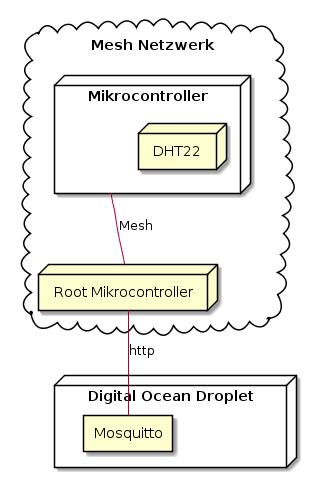
\includegraphics[scale=.5]{diagrams/mqtt_dht22_example_deployment.png}
        \caption{Deployment Diagramm (Quelle: eigene Darstellung)}
    \end{center}    
\end{figure}

In diesem kleinen Beispiel gibt es insgesamt 2 Mikrocontroller. 

\begin{itemize}
    \item Ein \textbf{Mikrocontroller} welcher mit einem DHT22 verbunden ist und regelmäßig die Sensordaten weiterschickt.
    \item Ein \textbf{Root Mikrocontroller} der nur für das weiterleiten der Nachrichten zuständig ist.
\end{itemize}

Der Root Mikrocontroller ist mit einem MQTT Broker (\textbf{Mosquitto}) verbunden.

Der \textbf{Mosquitto} Server läuft auf einer beliebigen \textbf{Host Machine} (Bsp.: Digital Ocean Droplet).

\vspace*{50px}
\begin{figure}[H]
    \begin{center}
        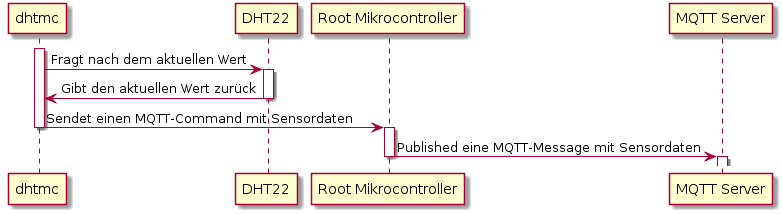
\includegraphics[scale=.5]{diagrams/mqtt_dht22_example_sequence.png}
        \caption{Sequence Diagramm (Quelle: eigene Darstellung)}
        \label{abb:dht22_sequence_diagram}
    \end{center}
\end{figure}
\vspace*{50px}

Die Abbildung \ref{abb:dht22_sequence_diagram} zeigt den Verlauf einer Iteration dieses Beispieles.
Der \textbf{dhtmc} (Der \textbf{Mikrocontroller} des Deployment Diagramms) ließt die aktuellen Werte des DHT22, welche er dann in dem Mesh Netzwerk mittels MQTT Command verschickt.

Wenn der \textbf{Root Mikrocontroller} diesen neuen MQTT Command bekommt schickt er die MQTT Nachricht an den angegebenen \textbf{MQTT Server} weiter.

Es wird davon ausgegangen, dass eine Installation von Nodejs mit einer Version von mindestens \textit{10} vorhanden ist.

Die Installation wird in Kapitel \ref{sec:nodejs} beschrieben.

\subsection{ESP-IDF Setup}

Die folgenden Anweisungen setzen ein Ubuntu-Betriebssystem vorraus. Es wird nicht garantiert, dass dies unter Alternativen wie zum Beispiel dem \textbf{Windows Subsystem for Linux (WSL) \ref{sec:wsl}} funktioniert. 

\subsubsection{Dependencies}

Zu aller erst müssen die Dependencies von ESP-IDF installiert werden. Dafür gibt es den folgenden shell command.

\vspace*{10px}
\begin{verbatim}
    sudo apt-get install git wget flex bison gperf python python-pip 
    python-setuptools cmake ninja-build ccache libffi-dev libssl-dev
\end{verbatim}
\vspace*{10px}

% TODO: install python3 things

\subsubsection{Libraries}

Damit man die ESP-IDF Libraries benutzen kann, muss man diese zuerst herunterladen.

\vspace*{10px}
\begin{verbatim}
    mkdir $HOME/esp &&
    cd $HOME/esp &&
    git clone --recursive https://github.com/espressif/esp-idf.git
\end{verbatim}
\vspace*{10px}

Mit den obigen Befehlen erstellt man zuerst einen neuen Ordner im Homeverzeichnis des aktuell eingeloggten Benutzer und wechselt in diesen. 
Anschließend wird das offizielle Repository von ESP-IDF rekursiv gecloned.

Nachdem das Repository erfolgreich gecloned wurde, muss man die Libraries installieren. Dies erfolgt durch folgende Bash Befehle.

\vspace*{10px}
\begin{verbatim}
    cd $HOME/esp/esp-idf &&
    ./install.sh
\end{verbatim}
\vspace*{10px}

Mit diesen Befehlen wird das Arbeitsverzeichnis auf das vorher installierte Repository gesetzt und die \textbf{install.sh} Datei von ESP-IDF ausgeführt.

Dies kann einige Minuten dauern.

\subsubsection{Umgebungsvariablen}

Damit die Toolchain nun verwendet werden kann, müssen noch ein paar Umgebungsvariablen definiert werden. 

\vspace*{10px}
\begin{verbatim}
    export IDF_PATH=$HOME/esp/esp-idf
\end{verbatim}
\vspace*{10px}

Die \textit{IDF\_PATH} Variable gibt den Pfad des Repositories von ESP-IDF an.

\vspace*{10px}
\begin{verbatim}
    . $HOME/esp/esp-idf/export.sh
\end{verbatim}
\vspace*{10px}

Danach müssen noch weitere Umgebungsvariablen von ESP-IDF selbst gesetzt werden, dafür muss man den oben angeführten Befehl ausführen.

Diese Variablen werden nur für die aktuelle Shell-Session gesetzt, deswegen wäre es sinnvoll diese Befehle in die \textbf{.bashrc} Datei im Homeverzeichnis zu schreiben.

\vspace*{10px}
\begin{verbatim}
    export IDF_PATH=$HOME/esp/esp-idf
    . $HOME/esp/esp-idf/export.sh
\end{verbatim}
\vspace*{10px}

Es ist auch möglich eine eigene Funktion dafür zu definieren, wenn man die Toolchain nur bei bedarf benutzen möchte.

\vspace*{10px}
\begin{verbatim}
    function loadEspIdf() {
        export IDF_PATH=$HOME/esp/esp-idf
        . $HOME/esp/esp-idf/export.sh
    }
\end{verbatim}
\vspace*{10px}

Anschließend muss der Terminal neugestartet werden, um die \textbf{.bashrc} Datei ausführen zu können.

\subsubsection{WSL}\label{sec:wsl}

WSL unterstützt bis zum Stand vom \textbf{29.03.2020} das Linux USB Interface nicht. Dies bedeutet, dass für eine fehlerfreie Nutzung der ESP-IDF-Toolchain nicht garantiert wird.

\subsection{Source Code}\label{sec:example-source-code}

Der Source Code der für dieses Beispiel benötigt wird, lebt in dem folgenden Repository.

\vspace*{10px}
\begin{verbatim}
    https://github.com/TimUntersberger/Diplomarbeit
\end{verbatim}
\vspace*{10px}

Für die erfolgreiche Absolvierung des Beispieles ist es notwendig das Repository zu clonen.

\vspace*{10px}
\begin{verbatim}
    git clone https://github.com/TimUntersberger/Diplomarbeit
\end{verbatim}
\vspace*{10px}

Nachdem der Command fertig ist, befinden sich mehrere Unterordner in dem neu erstellten Ordner namens \textit{Diplomarbeit}. Die einzigen relevanten Ordner für das Beispiel sind \textbf{Dht22Example} und \textbf{MeshVisualizer}.

Nach Bedarf können die anderen gelöscht werden.

Die zwei Dateien, welche in Kapitel \ref{sec:mosquitto} beschrieben werden, befinden sich in dem Unterordner \textbf{MeshVisualizer}.

Genauere Anweisungen zu \textbf{MeshVisualizer} befinden sich in dem Kapitel \ref{sec:example-mesh-visualizer}.

Die Struktur und wie der Code von \textbf{Dht22Example} benutzt werden kann, wird in dem Kapitel \ref{sec:code} beschrieben.

\subsection{Mosquitto}\label{sec:mosquitto}

\textbf{mosquitto.conf}
\begin{verbatim}
    listener 1883
    protocol mqtt

    listener 1884
    protocol websockets
\end{verbatim}
\vspace*{10px}

Die \textbf{mosquitto.conf} Datei konfiguriert den Mosquitto Broker so, dass er auf 2 Ports zu hört.

\begin{enumerate}
    \item 1883
    \item 1884
\end{enumerate}

Auf dem Port \textbf{1883} hört ein Websocket Server zu, welcher für die Nutzung von dem \textbf{Mesh Visualizer} \ref{sec:mesh-visualizer} konfiguriert wurde. 

Der Port 1883 ist wie üblich eine MQTT-Schnittstelle.

\textbf{docker-compose.yml}
\begin{verbatim}
    version: '3'
    services:
      mosquitto:
        image: eclipse-mosquitto
        ports:
          - '1883:1883'
          - '1884:1884'
        volumes:
            - ./mosquitto.conf:/mosquitto/config/mosquitto.conf
\end{verbatim}
\vspace*{10px}

Diese \textbf{docker-compose.yml} Datei verwendet die Version 3 von docker-compose. Insgesamt wird nur ein einziger Service benötigt für dieses Beispiel. Der Name des Services ist \textit{mosquitto} und benützt das offizielle Image von eclipse namens \textit{eclipse-mosquitto}.

Wie schon bei der \textbf{mosquitto.conf} Datei erwähnt, benötigt Mosquitto 2 offene Ports. Diese werden hier mit den selben äußeren Ports verbunden.

Die Konfigurationsdatei wird mittels eines Volumen in den Container injected.

In der folgenden Abbildung (\ref{abb:example_mosquitto_start}) ist zu sehen wie man den Mosquitto nun startet.

\begin{figure}[H]
    \begin{center}
        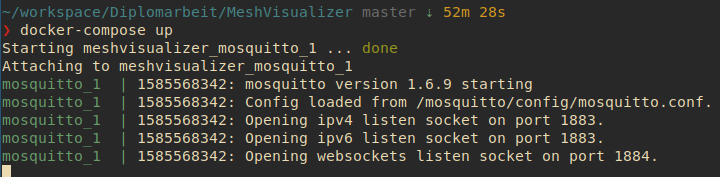
\includegraphics[scale=0.8]{images/example_mosquitto_start.png}
        \caption{Example Mosquitto Start (Quelle: eigene Darstellung)}
        \label{abb:example_mosquitto_start}
    \end{center}
\end{figure}

\subsection{Mesh Visualizer}\label{sec:example-mesh-visualizer}

Nach der erfolgreichen Absolvierung der in Kapitel \ref{sec:example-source-code} beschriebenen Anweisungen befindet sich nun der Unterordner namens \textbf{MeshVisualizer} in dem Ordner Diplomarbeit.

Bevor der \textbf{MeshVisualizer} gestartet werden kann, muss das Arbeitzverzeichnis auf den Pfad des \textbf{MeshVisualizer} Ordners gesetzt werden.

Anschließend ist es notwendig, die Dependencies des Projekts zu installieren.

Dies erfolgt durch den in Abbildung \ref{abb:example_mesh_visualizer_installation_cmd} angeführten Command.

\begin{figure}[H]
    \begin{center}
        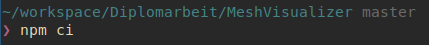
\includegraphics[scale=1]{images/example_mesh_visualizer_installation_cmd.png}
        \caption{Example Mesh Visualizer Installation Command (Quelle: eigene Darstellung)}
        \label{abb:example_mesh_visualizer_installation_cmd}
    \end{center}
\end{figure}

\pagebreak
In der nachstehenden Abbildung (\ref{abb:example_mesh_visualizer_installation_output}) wird das Ergebnis visualisiert.

\begin{figure}[H]
    \begin{center}
        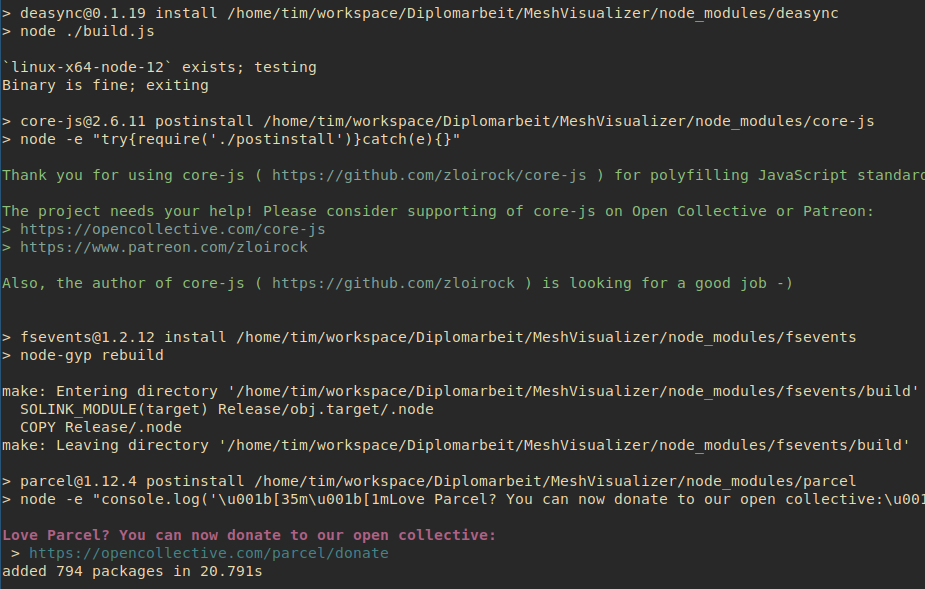
\includegraphics[scale=.6]{images/example_mesh_visualizer_installation_output.png}
        \caption{Example Mesh Visualizer Installation Output(Quelle: eigene Darstellung)}
        \label{abb:example_mesh_visualizer_installation_output}
    \end{center}
\end{figure}

Das starten des Visualizers geschieht wie in der nachstehenden Abbildung (\ref{abb:example_mesh_visualizer_start}).

\begin{figure}[H]
    \begin{center}
        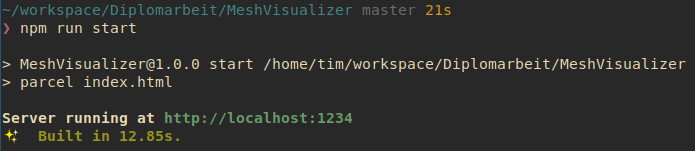
\includegraphics[scale=.6]{images/example_mesh_visualizer_start.png}
        \caption{Example Mesh Visualizer Start (Quelle: eigene Darstellung)}
        \label{abb:example_mesh_visualizer_start}
    \end{center}
\end{figure}

Nachdem der Server auf dem Port \textit{1234} läuft, ist nun die Website, welche in Abbildung \ref{abb:example_mesh_visualizer_website} zu sehen ist, auf der URL \textit{http://localhost:1234/} verfügbar.

\begin{figure}[H]
    \begin{center}
        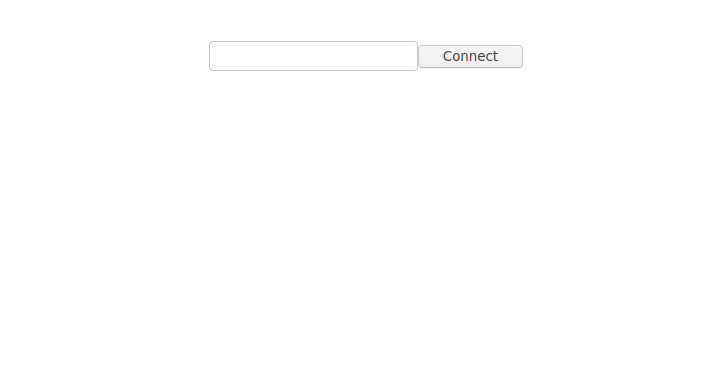
\includegraphics[scale=.3]{images/example_mesh_visualizer_website.png}
        \caption{Example Mesh Visualizer Website (Quelle: eigene Darstellung)}
        \label{abb:example_mesh_visualizer_website}
    \end{center}
\end{figure}

Auf der Website ist momentan nur ein Eingabefeld zusammen mit einem Knopf direkt daneben zu sehen.

Durch das Eingabefeld wird die URL des Mosquittos gesetzt. 
Die Definierung des verwendeten Protokolls darf nicht auser Acht gelassen werden.\newline

Da Javascript im Browser nicht in der Lage ist mit dem MQTT Protokoll zu kommunizieren, muss man sich mit dem vorher definierten Websocket Port (1884) des Brokers verbinden.

Beispiel
\begin{verbatim}
    ws://localhost:1884
\end{verbatim}

Mit dem Drücken des \textit{connect} Knopfs, wird versucht eine Verbindung mit dem Broker herzustellen.

Die Benutzung der Website wird in Kapitel \ref{sec:example-result} genauer erläutert.

\subsection{Config}

Die Konfiguration eines ESP-IDF Projekts, wird im Normfall mittels der menuconfig gelöst, wie in Kapitel \ref{sec:esp-idf-toolchain} erwähnt.

% TODO: write about required config values.

\subsection{Hardware}
% TODO: write about how to connect the dht22 with the esp
% TODO: write about how to connect the esp with the computer

\subsection{Hochladen}

Bevor das Programm auf den ESPs laufen kann, muss es hochgeladen werden.

Das Hochladen bzw. Flashen eines Programms verläuft wie in Kapitel \ref{sec:esp-idf-toolchain} beschrieben.

% TODO: fix dht2example program (only emit data if it is not root)

\subsection{Ergebnis}\label{sec:example-result}
\subsubsection{Mesh Visualizer}
\subsubsection{Mqtt Fx}
\subsection{Code}\label{sec:code}
\subsubsection{Struktur}
\subsubsection{Setup}
\subsubsection{IP Event Handler}
\subsubsection{Command Callback}
\subsubsection{DHT22 Task}
\subsection{Mögliche Probleme}
% TODO: Write about possible problems that could occur while following the example

% Installation der esp-idf toolchain
% Disclaimer: Wir nehmen "den" esp
% dht22 Beispiel vorstellen
%   deployment
%   sequence
% dht22 Anstecken
%   Welche Pins
%   Fertig angesteckten Esp herzeigen
% setup mosquitto (Mqtt)
%   websocket und mqtt
% setup mesh visualizer
% setup makeconfig
% Code
%   folder structure erklären
%   ip event handler erklären
%   command callback erklären
% Example Output herzeigen

\section{ELF vs. Bin}

\subsection{Bin}
Die Dateierweiterung .bin wird am häufigsten mit komprimierten Binärdateien verknüpft. Diese Dateien werden von vielen verschiedenen Computeranwendungen und für eine Vielzahl von Zwecken verwendet. Die Erweiterung .bin wird häufig für CD- und DVD-Backup-Image-Dateien verwendet.

In einigen Fällen werden die BIN-Dateien im einfachen Binärformat gespeichert und können mit einem Texteditor geöffnet werden. Es gibt jedoch einige BIN-Dateien, die von bestimmten Computeranwendungen erstellt werden und mit der Software geöffnet werden müssen, mit der sie erstellt wurden, oder mit einer kompatiblen Softwareanwendung.\cite{file.org_bin}

\subsection{Hintergrund}
Grundsätzlich sind Binärdateien als solche daran erkennbar, dass der Dateiinhalt, mit einem üblichen Texteditor angezeigt, keine oder überwiegend keine lesbaren Zeichen enthält. Der Versuch, eine Binärdatei als Textdatei zu interpretieren (beispielsweise durch Öffnen mit einem Texteditor), ergibt dann unleserlichen bzw. unsinnigen Text. Für die meisten der heute verwendeten 8-Bit-Zeichensätze gilt: nicht lesbare Steuerzeichen umfassen Zeichen mit ASCII-Werten von 0 bis 31, lesbare Zeichen die mit Werten von 32 bis 126. Die Lesbarkeit von Zeichen mit Werten ab 127 ist abhängig vom verwendeten Zeichensatz. Textdateien können auch gewisse Steuerzeichen enthalten, ohne dass sie deshalb als Binärdatei gelten; dazu gehören Steuerzeichen für Zeilenvorschub, Wagenrücklauf, Seitenumbruch (Seitenvorschub) und Tabulatorzeichen.

Weil Binärdateien alle möglichen Bit-Kombinationen nutzen, bieten sie eine höhere Informationsdichte als Textdateien. Deshalb benötigen sie meist weniger Speicherplatz auf Massenspeichern und lassen sich schneller laden und speichern. Ferner lassen sich darin verschiedene Objekttypen (beispielsweise Text mit Bildern) relativ einfach ablegen.

Binärformate werden beim Austausch über verschiedene Plattformen hinweg (beispielsweise Windows, Macintosh, Linux) nicht beschädigt, da die jeweiligen Softwarekomponenten nicht versuchen, die Dateien für die Zielplattform zu konvertieren. Andererseits wird der systemübergreifende Datenaustausch erschwert, da Binärdateien häufig Daten in einem systemabhängigen Format enthalten. (Beispielsweise Zahlen im Big- oder Little-Endian-Format.) Die Spezifikation des Dateiformats einer Binärdatei legt fest, wie mit der Datei zu verfahren ist. Zum Lesen, Bearbeiten und Speichern binärer Datenformate benötigt man im Allgemeinen spezielle, auf das Dateiformat abgestimmte Editoren (beispielsweise Textverarbeitung für Office-Texte, ein Bildbearbeitungsprogramm für Fotos, regedit für die Windows-Registrierungsdatenbank).

Zu beachten ist, dass man unter einer Binärdatei bzw. unter Binärformat nicht Daten versteht, die nur aus den (sichtbaren) Zeichen „0“ und „1“ aufgebaut sind – wie die Namensanalogie zu Hex(adezimal)datei nahelegen könnte. Binärdatei bedeutet auch nicht, dass die Daten nur aus binären „0“ und „1“ bestehen – weil das auch bei Text-Zeichensätzen der Fall ist. Auch ist eine Datei, die von einem Textverarbeitungsprogramm erzeugt wurde, meist (abhängig vom Dateiformat) keine reine Textdatei im engeren Sinn, sondern eine Binärdatei, in der zum Beispiel Formatangaben und andere Steuerzeichen nicht mit einem lesbaren Zeichensatz codiert sind. Solche Dateien, zum Beispiel im Rich-Text-Format, sind insofern eine Mischform aus Text- und Binärdatei.\cite{bin_wikipedia}

\subsection{ELF}
ELF ist die Abkürzung für Executable and Linkable Format und definiert die Struktur für Binärdateien, Bibliotheken und Core-Dateien. Die formale Spezifikation ermöglicht es dem Betriebssystem, die zugrunde liegenden Maschinenanweisungen korrekt zu interpretieren. ELF-Dateien sind normalerweise die Ausgabe eines Compilers oder Linkers und haben ein Binärformat.
\newline
\newline
Ein häufiges Missverständnis ist, dass ELF-Dateien nur für Binärdateien oder ausführbare Dateien bestimmt sind. Es ist jedoch möglich sie für Teilstücke (Objektcode) verwendet zu können. Ein weiteres Beispiel sind gemeinsam genutzte Bibliotheken oder sogar Core-Dumps (Core- oder a.out-Dateien). Die ELF-Spezifikation wird auch unter Linux für den Kernel selbst und die Linux-Kernelmodule verwendet.


\subsection{Struktur}
Aufgrund des erweiterbaren Designs von ELF-Dateien unterscheidet sich die Struktur je nach Datei. Eine ELF-Datei besteht aus:

\begin{itemize} 
\item ELF-Header
\item Dateidaten
\end{itemize}

Mit dem Befehl readelf können wir uns die Struktur einer Datei ansehen und sie sieht ungefähr so aus:

\begin{figure}[H]
    \begin{center}
        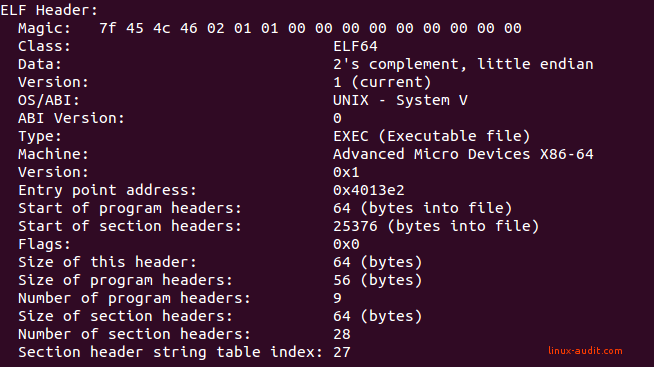
\includegraphics[scale=0.5]{images/elf-header-linux-binary.png}
        \caption{Details einer Elf-binary \cite{details_of_Elf_binary}}
    \end{center}
\end{figure}
 
\subsection{ELF-Header}
Wie in diesem Screenshot zu sehen ist, beginnt der ELF-Header mit etwas Magic. Diese ELF-Header-Magic liefert Informationen über die Datei. Die ersten 4 hexadezimalen Teile definieren, dass dies eine ELF-Datei ist (45 = E, 4c = L, 46 = F), der der Wert 7f vorangestellt ist.
 
Dieser ELF-Header ist obligatorisch. Es stellt sicher, dass Daten während der Verknüpfung oder Ausführung korrekt interpretiert werden. Um die innere Funktionsweise einer ELF-Datei besser zu verstehen, ist es hilfreich zu wissen, dass diese Header-Informationen verwendet werden.
 
\subsubsection{Class}
Nach der ELF-Typdeklaration ist ein Class-feld definiert. Dieser Wert bestimmt die Architektur für die Datei. Es kann sich um eine 32-Bit- (= 01) oder 64-Bit- (= 02) Architektur handeln. Magic zeigt eine 02, die vom Befehl readelf als ELF64-Datei übersetzt wird. Mit anderen Worten, eine ELF-Datei, die die 64-Bit-Architektur verwendet.

\subsubsection{Data}
Der nächste Teil ist das Data-feld. Es kennt zwei Optionen: 01 für LSB (Least Significant Bit), auch als Little-Endian bekannt. Dann gibt es den Wert 02 für MSB (Most Significant Bit, Big-Endian). Dieser spezielle Wert hilft dabei, die verbleibenden Objekte in der Datei korrekt zu interpretieren. Dies ist wichtig, da verschiedene Prozessortypen unterschiedlich mit den eingehenden Anweisungen und Datenstrukturen umgehen. In diesem Fall wird LSB verwendet, was für Prozessoren vom Typ AMD64 üblich ist.

\subsubsection{Version}
Als nächstes folgt eine weitere "01" in der Magic, die die Versionsnummer ist. Derzeit gibt es nur einen Versionstyp: Derzeit ist dies der Wert "01". Also nichts Interessantes zu merken.

\subsubsection{OS / ABI}
Jedes Betriebssystem hat eine große Überlappung in gemeinsamen Funktionen. Darüber hinaus hat jedes von ihnen spezifische oder zumindest geringfügige Unterschiede. Die Definition des richtigen Sets erfolgt über eine Application Binary Interface (ABI). Auf diese Weise wissen sowohl das Betriebssystem als auch die Anwendungen, was zu erwarten ist, und die Funktionen werden korrekt weitergeleitet. Diese beiden Felder beschreiben, für was ABI verwendet wird und die zugehörige Version. In diesem Fall ist der Wert 00, was bedeutet, dass keine bestimmte Erweiterung verwendet wird. Die Ausgabe zeigt dies als System V.

\subsubsection{ABI-Version}
Bei Bedarf kann eine Version für das ABI angegeben werden.

\subsubsection{Machine}
Den Maschinentyp (AMD64) finden wir auch im Header.

\subsubsection{Type}
Das Typfeld gibt an, wozu die Datei dient. Es gibt einige gängige Dateitypen.

\begin{itemize}
\item CORE (Wert 4)
\item DYN (Shared Object File) für Bibliotheken (Wert 3)
\item EXEC (ausführbare Datei) für Binärdateien (Wert 2)
\item REL (verschiebbare Datei), bevor sie in eine ausführbare Datei gelinked wird (Wert 1)
\end{itemize}

\subsection{File Data}
Neben dem ELF-Header bestehen ELF-Dateien aus drei Teilen.

\begin{itemize}
\item Program Headers oder Segments (9)
\item Section Headers oder Sections (28)
\item Data
\end{itemize}

Außerdem ist es gut zu wissen, dass ELF zwei sich ergänzende „Ansichten“ hat. Eine Benutzeroberfläche muss für den Linker verwendet werden, um die Ausführung zu ermöglichen (segments). Die andere zum Kategorisieren von Anweisungen und Daten (sections). Je nach Ziel werden also die zugehörigen Headertypen verwendet.

\subsubsection{Programm-Header}
Eine ELF-Datei besteht aus null oder mehr Segmenten und beschreibt, wie ein process/memory image für die Laufzeitausführung erstellt wird. Wenn der Kernel diese Segmente sieht, verwendet er sie, um sie mithilfe des Systemaufrufs mmap (2) dem virtuellen Adressraum zuzuordnen. Mit anderen Worten, es konvertiert vordefinierte Anweisungen in ein Speicherbild. Wenn Ihre ELF-Datei eine normale Binärdatei ist, sind diese Programmheader erforderlich. Andernfalls wird es einfach nicht ausgeführt. Diese Header mit der zugrunde liegenden Datenstruktur werden verwendet, um einen Prozess zu bilden. Dieser Vorgang ist für shared libraries ähnlich.

\begin{figure}[H]
    \begin{center}
        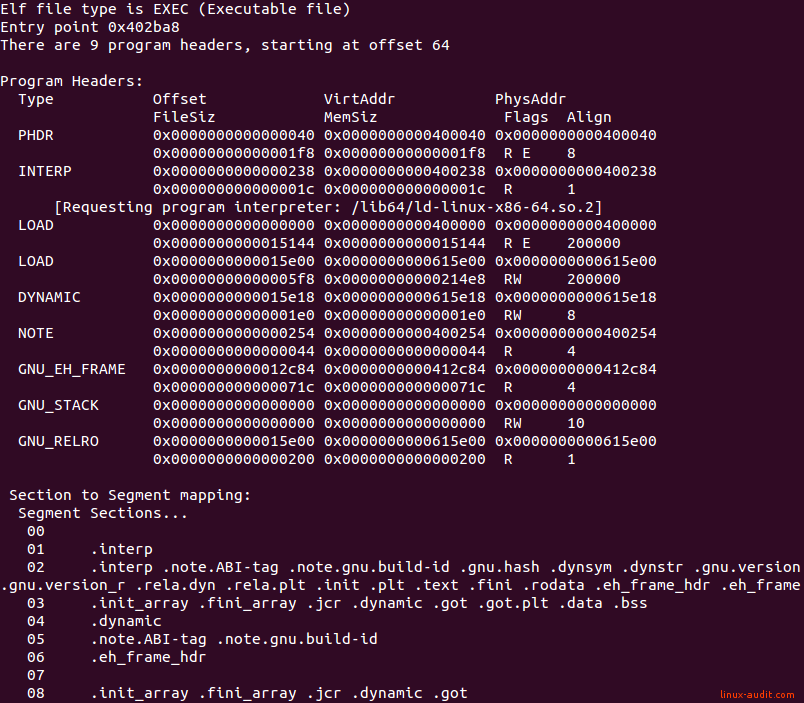
\includegraphics[scale=0.5]{images/elf-program-headers-segments.png}
        \caption{Programm Header einer Elf binary \cite{program_headers_of_Elf_binary}}
    \end{center}
\end{figure}

\subsubsection{GNU\_EH\_FRAME}
Dies ist eine sorted queue, die vom GNU C-Compiler (gcc) verwendet wird. Es speichert Ausnahmebehandlungsroutinen. Wenn also etwas schief geht, kann es diesen Bereich verwenden, um richtig damit umzugehen.

\subsubsection{GNU\_STACK}
Dieser Header wird zum Speichern von stack-Informationen verwendet. Der stack ist ein Puffer oder eine Arbeitsstelle, an der Elemente wie lokale Variablen gespeichert werden. Dies geschieht bei LIFO (Last In, First Out). Beim Starten einer Prozessfunktion wird ein Baustein reserviert. Wenn die Funktion beendet ist, wird sie wieder als frei markiert. Der interessante Teil ist nun, dass ein Stack nicht ausführbar sein sollte, da dies zu Sicherheitslücken führen kann. Durch Manipulation des Speichers könnte man auf diesen ausführbaren stack verweisen und beabsichtigte Anweisungen ausführen.

Wenn das Segment GNU\_STACK nicht verfügbar ist, wird normalerweise ein executable stack verwendet.
Die Tools scanelf und execstack sind zwei Beispiele, um die stack-Details anzuzeigen.

\begin{figure}[H]
    \begin{center}
        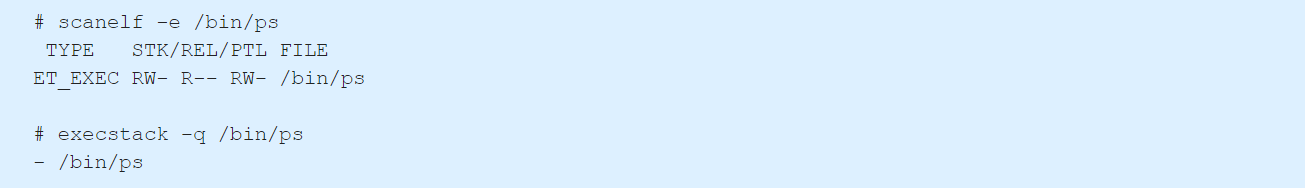
\includegraphics[scale=1]{images/example_gnustack.png}
        \caption{Beispiel GNU\_STACK \cite{example_gnustack}}
    \end{center}
\end{figure}

\subsection{Static vs. Daynamic binaries}
Beim Umgang mit ELF-Binärdateien ist es gut zu wissen, dass es zwei Typen gibt und wie sie verknüpft sind. Der Typ ist entweder statisch oder dynamisch und bezieht sich auf die verwendeten Bibliotheken. Zu Optimierungszwecken stellen wir häufig fest, dass Binärdateien „dynamisch“ sind, was bedeutet, dass externe Komponenten für die ordnungsgemäße Ausführung erforderlich sind. Häufig handelt es sich bei diesen externen Komponenten um normale Bibliotheken, die allgemeine Funktionen wie das Öffnen von Dateien oder das Erstellen eines Netzwerk-Sockets enthalten. In statischen Binärdateien sind dagegen alle Bibliotheken enthalten. Dadurch werden sie größer und dennoch tragbarer (z. B. wenn sie auf einem anderen System verwendet werden).

\subsection{Fazit}
ELF-Dateien dienen zur Ausführung oder zum Verknüpfen. Abhängig vom primären Ziel enthält es die erforderlichen Segmente oder Abschnitte. Segmente werden vom Kernel angeschaut und auf den Speicher gemappt (mithilfe von mmap). Abschnitte werden vom Linker angeschaut, um ausführbaren Code oder freigegebene Objekte zu erstellen.

Der ELF-Dateityp ist sehr flexibel und bietet Unterstützung für mehrere CPU-Typen, Maschinenarchitekturen und Betriebssysteme. Es ist auch sehr erweiterbar: Jede Datei ist je nach den erforderlichen Teilen unterschiedlich aufgebaut.

Header bilden einen wichtigen Teil der Datei und beschreiben genau den Inhalt einer ELF-Datei. Mit den richtigen Tools erhalten Sie ein grundlegendes Verständnis des Zwecks der Datei. Von dort aus können Sie die Binärdateien weiter überprüfen. Dies kann durch Bestimmen der zugehörigen Funktionen oder der in der Datei gespeicherten Zeichenfolgen erfolgen.\cite{elf_linux_audit}
% create further tex files for all other chapters of your document
\chapter{Resümee}
%TODO technisch ziele, was wurde erreicht
%todo hardware anders zu arbeiten

\section{Tim Untersberger}
%todo ändern

Im Laufe dieser Arbeit habe ich das Arbeiten mit Mikrocontrollern näher kennengelernt und meine C/C++ verfeinern dürfen.

Durch diese Arbeit durfte ich in die Welt der Mikrocontroller eintretten, was mir die Augen für neue Möglichkeiten geöffnet hat. Am Anfag war es nicht leicht mit Mikrocontrollern zu arbeiten, da das Arbeiten mit Mikrocontrollern sehr stark von dem ,was wir in unseren Schulstunden gelernt haben, abschweift.

Das Zusammenarbeiten mit einem Partner war am Anfang eine kleine Herausforderung, welche aber zum Glück schnell Überwunden wurde.

Diese Diplomarbeit hat mir einige Dinge im Thema Zeitmanagement beigebracht und ich werde diese Erfahrung mein Leben lang schätzen.

\section{Stefan Waldl}
Beim Arbeiten an dieser Diplomarbeit konnte ich viel für mein Leben lernen. Der größte Punkt, was das betrifft, war das Arbeiten mit einem Partner. Man lernt, wie wichtig es ist einfach aber trotzdem prägnant zu kommunizieren, da sonst bei einem größeren Projekt wie diesem leicht Missverständnise auftreten können.

Anfangs war es sehr mühsam, auf Mikrocontrollern zu programmieren, da sich diese ganz anders verhalten als herkömmliche Computer. Doch als ich mich an die Eigenheiten der Mikrocontrollern gewöhnt hatte, war es auch mir möglich, in einen produktiven Workflow zu gelangen.

Im Großen und Ganzen bin ich froh, mein Know-How um die Welt der Mikrocontroller erweitern haben zu können.

\bibliography{da_bibliography}{}
\bibliographystyle{plainurl} % alternatives plainurl, alphaurl;  german alternative: dinat (but add package natbib)

\listoffigures
\listoftables
\chapter*{Project Log Book}
\begin{tabular}{|l|l|l|l|}
\hline
Date & Participants & Todos & Due\\
\hline
\end{tabular}

\appendix
\chapter{Additional Information} \label{cha:additional-information}
If needed the appendix is the place where additional information concerning your thesis goes. Examples could be:
\begin{itemize}
	\item Source Code
	\item Test Protocols
	\item Project Proposal
	\item Project Plan
	\item Individual Goals
	\item \ldots
\end{itemize}
Again this has to be aligned with the supervisor.
%\chapter{Individual Goals} \label{cha:individual-goals}
This is just another example to show what content could go into the appendix.
\end{document}  